% Meta-Informationen -------------------------------------------------------
%		Informationen über das Dokument, wie z.B. Titel, Autor, Matrikelnr. etc
%		werden in der Datei _Meta.tex definiert und können danach global
%		verwendet werden.
% --------------------------------------------------------------------------
% Informationen ------------------------------------------------------------
% 	Definition von globalen Parametern, die im gesamten Dokument verwendet
% 	werden können (z.B auf dem Deckblatt etc.).
% --------------------------------------------------------------------------
\newcommand{\titel}{End-to-End Reinforcement Learning Training of a Convolutional Neural Network to achieve an autonomous driving agent resilient to light changes}
\newcommand{\art}{Master's Thesis}
\newcommand{\ort}{Leipzig}
\newcommand{\hochschule}{Universität Leipzig}
\newcommand{\fachgebiet}{Database Department}
\newcommand{\fakultaet}{Faculty of Mathematics and Computer Science}
\newcommand{\institut}{Institute of Computer Science}
\newcommand{\autor}{Georg Schneeberger}
\newcommand{\matrikelnr}{3707914}
\newcommand{\erstbetreuer}{Prof. Dr. Erhard Rahm}
\newcommand{\zweitbetreuer}{Dr. Thomas Burghardt}
\newcommand{\drittbetreuer}{Martin Lorenz}
\newcommand{\jahr}{2024}
\newcommand{\invnr}{1337}
\newcommand{\eingereicht}{28.06.2024}

% Eigene Befehle
\newcommand{\todo}[1]{\textbf{\textsc{\textcolor{red}{(TODO: #1)}}}}

% Autorennamen in small caps
\newcommand{\AutorZ}[1]{\textsc{#1}}
\newcommand{\Autor}[1]{\AutorZ{\citeauthor{#1}}}

% Befehle zur semantischen Auszeichnung von Text
\newcommand{\NeuerBegriff}[1]{\textbf{#1}}
\newcommand{\Fachbegriff}[1]{\textit{#1}}
\newcommand{\Prozess}[1]{\textit{#1}}
\newcommand{\Webservice}[1]{\textit{#1}}
\newcommand{\Eingabe}[1]{\texttt{#1}}
\newcommand{\Code}[1]{\texttt{#1}}
\newcommand{\Datei}[1]{\texttt{#1}}
\newcommand{\Datentyp}[1]{\textsf{#1}}
\newcommand{\XMLElement}[1]{\textsf{#1}}

% Abkürzungen
\newcommand{\vgl}{Vgl.\ }
\newcommand{\ua}{\mbox{u.\,a.\ }}
\newcommand{\zB}{\mbox{z.\,B.\ }}
\newcommand{\bs}{$\backslash$}

% Einfache Anführungszeichen in texttt
\newcommand{\sq}{\textquotesingle}



% Dokumentenkopf -----------------------------------------------------------
% 	Diese Vorlage basiert auf "scrreprt" aus dem koma-script.
%		Die Option draft sollte beim fertigen Dokument ausgeschaltet werden.
% --------------------------------------------------------------------------
\documentclass[
	11pt,					% Schriftgröße
	DIV=10,
	%ngerman,				% für Umlaute, Silbentrennung etc.
	english,
	a4paper,				% Papierformat
	oneside,				% einseitiges Dokument
	titlepage,				% es wird eine Titelseite verwendet
	parskip=half,			% Abstand zwischen Absätzen (halbe Zeile)
	headings=normal, % Größe der Überschriften verkleinern
	numbers=withendperiod, % Fügt in den Überschriften nach den Zahlen einen Punkt ein
	listof=totoc,				% Verzeichnisse im Inhaltsverzeichnis aufführen
	bibliography=totoc,				% Literaturverzeichnis im Inhaltsverzeichnis aufführen
	index=totoc,				% Index im Inhaltsverzeichnis aufführen
	captions=tableheading,		% Beschriftung von Tabellen oberhalb ausgeben
	final					% Status des Dokuments (final/draft)
]{scrreprt}

\renewcommand*\chapterheadstartvskip{\vspace*{-1.0cm}}

% Bentigte Packages -------------------------------------------------------
%		Weitere Packages, die benötigt werden, sind in die Datei Packages.tex
%		"ausgelagert", um die Vorlage möglichst übersichtlich zu halten.
% --------------------------------------------------------------------------
%% Anpassung des Seitenlayouts ----------------------------------------------
% 	siehe Seitenstil.tex
% --------------------------------------------------------------------------
\usepackage[
	automark,			% Kapitelangaben in Kopfzeile automatisch erstellen
	headsepline,	% Trennlinie unter Kopfzeile
	ilines				% Trennlinie linksbündig ausrichten
]{scrlayer-scrpage}
\usepackage{scrhack} % Disable some warnings

\usepackage{pseudocode}
\usepackage{nicefrac}

% Für eine schöne Anordnung von Bildern
\usepackage{subfigure}

\usepackage{dsfont}
%\usepackage{color}
%
%% Define user colors using the RGB model
%\definecolor{yellow}{rgb}{0.0,1.0,0.0}
%\definecolor{rot}{rgb}{1.0,0.0,0.0}

% Anpassung an Landessprache -----------------------------------------------
% 	Verwendet globale Option german siehe \documentclass
% --------------------------------------------------------------------------
\usepackage[ngerman]{babel}

% Umlaute ------------------------------------------------------------------
% 		Umlaute/Sonderzeichen wie äöüß direkt im Quelltext verwenden (CodePage).
%		Erlaubt automatische Trennung von Worten mit Umlauten.
% --------------------------------------------------------------------------
\usepackage[utf8]{inputenc}
\usepackage[T1]{fontenc}
%\usepackage{ae} % "schöneres" ä
\usepackage{textcomp} % Euro-Zeichen etc.
\usepackage{lmodern} % schööön

% Grafiken -----------------------------------------------------------------
% 		Einbinden von Grafiken [draft oder final]
% 		Option [draft] bindet Bilder nicht ein - auch globale Option
% --------------------------------------------------------------------------
\usepackage[dvips,final]{graphicx}
\usepackage{wrapfig}
\graphicspath{{Bilder/}} % Dort liegen die Bilder des Dokuments

% Befehle aus AMSTeX für mathematische Symbole z.B. \boldsymbol \mathbb ----
\usepackage{amsmath,amsfonts,amsthm}

% Für Index-Ausgabe; \printindex -------------------------------------------
\usepackage{makeidx}

% Einfache Definition der Zeilenabstände und Seitenränder etc. -------------
\usepackage{setspace}
\usepackage{geometry}

% für gedrehte Tabellen
\usepackage{rotating} 

% Symbolverzeichnis --------------------------------------------------------
% 	Symbolverzeichnisse bequem erstellen, beruht auf MakeIndex.
% 		makeindex.exe %Name%.nlo -s nomencl.ist -o %Name%.nls
% 	erzeugt dann das Verzeichnis. Dieser Befehl kann z.B. im TeXnicCenter
%		als Postprozessor eingetragen werden, damit er nicht ständig manuell
%		ausgeführt werden muss.
%		Die Definitionen sind ausgegliedert in die Datei Abkuerzungen.tex.
% --------------------------------------------------------------------------
\usepackage[intoc]{nomencl}
  \let\abbrev\nomenclature
  \renewcommand{\nomname}{Abkürzungsverzeichnis}
  \setlength{\nomlabelwidth}{.25\hsize}
  \renewcommand{\nomlabel}[1]{#1 \dotfill}
  \setlength{\nomitemsep}{-\parsep}

% Zum Umfließen von Bildern -------------------------------------------------
\usepackage{floatflt}

% Zum Einbinden von Programmcode --------------------------------------------
\usepackage{listings}
\usepackage{xcolor} 
\definecolor{hellgelb}{rgb}{1,1,0.9}
\definecolor{colKeys}{rgb}{0,0,1}
\definecolor{colIdentifier}{rgb}{0,0,0}
\definecolor{colComments}{rgb}{1,0,0}
\definecolor{colString}{rgb}{0,0.5,0}
\lstset{%
    float=hbp,%
    basicstyle=\texttt\small, %
    identifierstyle=\color{colIdentifier}, %
    keywordstyle=\color{colKeys}, %
    stringstyle=\color{colString}, %
    commentstyle=\color{colComments}, %
    columns=flexible, %
    tabsize=2, %
    frame=single, %
    extendedchars=true, %
    showspaces=false, %
    showstringspaces=false, %
    numbers=left, %
    numberstyle=\tiny, %
    breaklines=true, %
    backgroundcolor=\color{hellgelb}, %
    breakautoindent=true, %
%    captionpos=b%
}

% Lange URLs umbrechen etc. -------------------------------------------------
\usepackage{url}


\usepackage{makecell}

%% Wichtig für korrekte Zitierweise ------------------------------------------

\usepackage[autocite=inline, sorting=none]{biblatex}
\bibliography{quellen} % Name der .bib-Datei

\usepackage{csquotes} % Empfohlen, um Zitierten Text richtig darzustellen

% ermöglicht Zeilenumbrüche in Captions
\usepackage{caption}


% PDF-Optionen --------------------------------------------------------------
\usepackage[
bookmarks,
bookmarksopen=true,
pdftitle={\titel},
pdfauthor={\autor},
pdfcreator={\autor},
pdfsubject={\titel},
pdfkeywords={\titel},
colorlinks=true,
%linkcolor=red, % einfache interne Verknüpfungen
%anchorcolor=black,% Ankertext
%citecolor=blue, % Verweise auf Literaturverzeichniseinträge im Text
%filecolor=magenta, % Verknüpfungen, die lokale Dateien öffnen
%menucolor=red, % Acrobat-Menüpunkte
%urlcolor=cyan, 
% für die Druckversion können die Farben ausgeschaltet werden:
linkcolor=black, % einfache interne Verknüpfungen
anchorcolor=black,% Ankertext
citecolor=black, % Verweise auf Literaturverzeichniseinträge im Text5
filecolor=black, % Verknüpfungen, die lokale Dateien öffnen
menucolor=black, % Acrobat-Menüpunkte
urlcolor=black, 
%backref,
%pagebackref,
plainpages=false,% zur korrekten Erstellung der Bookmarks
pdfpagelabels,% zur korrekten Erstellung der Bookmarks
hypertexnames=false,% zur korrekten Erstellung der Bookmarks
linktocpage % Seitenzahlen anstatt Text im Inhaltsverzeichnis verlinken
]{hyperref}

% Zum fortlaufenden Durchnummerieren der Fußnoten ---------------------------
\usepackage{chngcntr}


% für lange Tabellen
\usepackage{longtable}
\usepackage{array}
\usepackage{ragged2e}
\usepackage{lscape}

\usepackage{supertabular}

% Spaltendefinition rechtsbündig mit definierter Breite ---------------------
\newcolumntype{w}[1]{>{\raggedleft\hspace{0pt}}p{#1}}

% Formatierung von Listen ändern
\usepackage{paralist}
% Standardeinstellungen:
% \setdefaultleftmargin{2.5em}{2.2em}{1.87em}{1.7em}{1em}{1em}

\usepackage{tablefootnote}
% für Ausblenden der Seitenzahl
\usepackage{lipsum}
% Anpassung des Seitenlayouts ----------------------------------------------
% 	siehe Seitenstil.tex
% --------------------------------------------------------------------------
\usepackage[
	automark,			% Kapitelangaben in Kopfzeile automatisch erstellen
	headsepline,	% Trennlinie unter Kopfzeile
	ilines				% Trennlinie linksbündig ausrichten
]{scrlayer-scrpage}
\usepackage{scrhack} % Disable some warnings

\usepackage{pseudocode}
\usepackage{nicefrac}

% Für eine schöne Anordnung von Bildern
\usepackage{subfigure}

\usepackage{dsfont}
%\usepackage{color}
%
%% Define user colors using the RGB model
%\definecolor{yellow}{rgb}{0.0,1.0,0.0}
%\definecolor{rot}{rgb}{1.0,0.0,0.0}

% Anpassung an Landessprache -----------------------------------------------
% 	Verwendet globale Option german siehe \documentclass
% --------------------------------------------------------------------------
\usepackage[ngerman]{babel}

% Umlaute ------------------------------------------------------------------
% 		Umlaute/Sonderzeichen wie äöüß direkt im Quelltext verwenden (CodePage).
%		Erlaubt automatische Trennung von Worten mit Umlauten.
% --------------------------------------------------------------------------
\usepackage[utf8]{inputenc}
\usepackage[T1]{fontenc}
%\usepackage{ae} % "schöneres" ä
\usepackage{textcomp} % Euro-Zeichen etc.
\usepackage{lmodern} % schööön

% Grafiken -----------------------------------------------------------------
% 		Einbinden von Grafiken [draft oder final]
% 		Option [draft] bindet Bilder nicht ein - auch globale Option
% --------------------------------------------------------------------------
\usepackage[dvips,final]{graphicx}
\usepackage{wrapfig}
\graphicspath{{Bilder/}} % Dort liegen die Bilder des Dokuments

% Befehle aus AMSTeX für mathematische Symbole z.B. \boldsymbol \mathbb ----
\usepackage{amsmath,amsfonts,amsthm}

% Für Index-Ausgabe; \printindex -------------------------------------------
\usepackage{makeidx}

% Einfache Definition der Zeilenabstände und Seitenränder etc. -------------
\usepackage{setspace}
\usepackage{geometry}

% für gedrehte Tabellen
\usepackage{rotating} 

% Symbolverzeichnis --------------------------------------------------------
% 	Symbolverzeichnisse bequem erstellen, beruht auf MakeIndex.
% 		makeindex.exe %Name%.nlo -s nomencl.ist -o %Name%.nls
% 	erzeugt dann das Verzeichnis. Dieser Befehl kann z.B. im TeXnicCenter
%		als Postprozessor eingetragen werden, damit er nicht ständig manuell
%		ausgeführt werden muss.
%		Die Definitionen sind ausgegliedert in die Datei Abkuerzungen.tex.
% --------------------------------------------------------------------------
\usepackage[intoc]{nomencl}
  \let\abbrev\nomenclature
  \renewcommand{\nomname}{Abkürzungsverzeichnis}
  \setlength{\nomlabelwidth}{.25\hsize}
  \renewcommand{\nomlabel}[1]{#1 \dotfill}
  \setlength{\nomitemsep}{-\parsep}

% Zum Umfließen von Bildern -------------------------------------------------
\usepackage{floatflt}

% Zum Einbinden von Programmcode --------------------------------------------
\usepackage{listings}
\usepackage{xcolor} 
\definecolor{hellgelb}{rgb}{1,1,0.9}
\definecolor{colKeys}{rgb}{0,0,1}
\definecolor{colIdentifier}{rgb}{0,0,0}
\definecolor{colComments}{rgb}{1,0,0}
\definecolor{colString}{rgb}{0,0.5,0}
\lstset{%
    float=hbp,%
    basicstyle=\texttt\small, %
    identifierstyle=\color{colIdentifier}, %
    keywordstyle=\color{colKeys}, %
    stringstyle=\color{colString}, %
    commentstyle=\color{colComments}, %
    columns=flexible, %
    tabsize=2, %
    frame=single, %
    extendedchars=true, %
    showspaces=false, %
    showstringspaces=false, %
    numbers=left, %
    numberstyle=\tiny, %
    breaklines=true, %
    backgroundcolor=\color{hellgelb}, %
    breakautoindent=true, %
%    captionpos=b%
}

% Lange URLs umbrechen etc. -------------------------------------------------
\usepackage{url}


\usepackage{makecell}

%% Wichtig für korrekte Zitierweise ------------------------------------------

\usepackage[autocite=inline, sorting=none]{biblatex}
\bibliography{quellen} % Name der .bib-Datei

\usepackage{csquotes} % Empfohlen, um Zitierten Text richtig darzustellen

% ermöglicht Zeilenumbrüche in Captions
\usepackage{caption}


% PDF-Optionen --------------------------------------------------------------
\usepackage[
bookmarks,
bookmarksopen=true,
pdftitle={\titel},
pdfauthor={\autor},
pdfcreator={\autor},
pdfsubject={\titel},
pdfkeywords={\titel},
colorlinks=true,
%linkcolor=red, % einfache interne Verknüpfungen
%anchorcolor=black,% Ankertext
%citecolor=blue, % Verweise auf Literaturverzeichniseinträge im Text
%filecolor=magenta, % Verknüpfungen, die lokale Dateien öffnen
%menucolor=red, % Acrobat-Menüpunkte
%urlcolor=cyan, 
% für die Druckversion können die Farben ausgeschaltet werden:
linkcolor=black, % einfache interne Verknüpfungen
anchorcolor=black,% Ankertext
citecolor=black, % Verweise auf Literaturverzeichniseinträge im Text5
filecolor=black, % Verknüpfungen, die lokale Dateien öffnen
menucolor=black, % Acrobat-Menüpunkte
urlcolor=black, 
%backref,
%pagebackref,
plainpages=false,% zur korrekten Erstellung der Bookmarks
pdfpagelabels,% zur korrekten Erstellung der Bookmarks
hypertexnames=false,% zur korrekten Erstellung der Bookmarks
linktocpage % Seitenzahlen anstatt Text im Inhaltsverzeichnis verlinken
]{hyperref}

% Zum fortlaufenden Durchnummerieren der Fußnoten ---------------------------
\usepackage{chngcntr}


% für lange Tabellen
\usepackage{longtable}
\usepackage{array}
\usepackage{ragged2e}
\usepackage{lscape}

\usepackage{supertabular}

% Spaltendefinition rechtsbündig mit definierter Breite ---------------------
\newcolumntype{w}[1]{>{\raggedleft\hspace{0pt}}p{#1}}

% Formatierung von Listen ändern
\usepackage{paralist}
% Standardeinstellungen:
% \setdefaultleftmargin{2.5em}{2.2em}{1.87em}{1.7em}{1em}{1em}

\usepackage{tablefootnote}
% für Ausblenden der Seitenzahl
\usepackage{lipsum}

% Erstellung eines Index und Abkürzungsverzeichnisses aktivieren -----------
\makeindex
% makeindex Masterarbeit.nlo -s nomencl.ist -o Masterarbeit.nls
\makenomenclature


% Kopf- und Fußzeilen, Seitenränder etc. -----------------------------------
% Zeilenabstand ------------------------------------------------------------
\onehalfspacing 
% \setstretch{1,5}

% Seitenränder -------------------------------------------------------------
\geometry{paper=a4paper,left=25mm,right=20mm,top=20mm, bottom=25mm}
% Notfall maße :)
%\geometry{paper=a4paper,left=35mm,right=25mm,top=25mm, bottom=25mm}



% Kopf- und Fußzeilen ------------------------------------------------------
\pagestyle{scrheadings}

% Kopf- und Fußzeile auch auf Kapitelanfangsseiten -------------------------
\renewcommand*{\chapterpagestyle}{scrheadings}

% Schriftform der Kopfzeile ------------------------------------------------
\renewcommand{\headfont}{\normalfont}

% Kopfzeile ----------------------------------------------------------------
\ihead{\textit{\headmark}}
\chead{}
%\ohead{\includegraphics[scale=1]{Bilder/logoKlein.JPG}}
\ohead{}
\setlength{\headheight}{8mm} % Höhe der Kopfzeile
\setheadwidth[0pt]{textwithmarginpar} % Kopfzeile über den Text hinaus verbreitern

% Fußzeile -----------------------------------------------------------------
% \ifoot{\copyright\ \autor \\ \invnr}
% \ifoot{\copyright\ \autor \\ \matrikelnr}
\ifoot{\autor \\ \matrikelnr}
\cfoot{}
\ofoot{\pagemark}
\setlength{\footskip}{12mm}
\setfootwidth[0pt]{text}

% Überschriften ------------------------------------------------------------
\renewcommand*\chapterheadstartvskip{\vspace*{-0.5cm}} % Platz vor einer Überschrift eines neuen Kapitels


% erzeugt ein wenig mehr Platz hinter einem Punkt --------------------------
\frenchspacing

% Schusterjungen und Hurenkinder vermeiden
\clubpenalty = 10000
\widowpenalty = 10000 
\displaywidowpenalty = 10000


% Quellcode-Ausgabe formatieren --------------------------------------------
%\lstset{numbers=left, numberstyle=\tiny, numbersep=5pt, breaklines=true}
%\lstset{emph={square}, emphstyle=\color{red}, emph={[2]root,base}, emphstyle={[2]\color{blue}}}

\definecolor{gray}{rgb}{0.9,0.9,0.9}

\lstset{%
		basicstyle=\small\ttfamily,language={[LaTeX]TeX},
		numbersep=5mm, 
		numbers=left,
		numberstyle=\tiny,
		breaklines=true,
		framexleftmargin=8mm, 
		xleftmargin=8mm,
		backgroundcolor=\color{gray},
		captionpos=b
}%

% Fußnoten fortlaufend durchnummerieren ------------------------------------
\counterwithout{footnote}{chapter}

% Definitionen

\newtheorem{definition}{Definition}


% Eigene Definitionen für Silbentrennung
\hyphenation{Trenn-bar-es}

% Das eigentliche Dokument -------------------------------------------------
%		Der eigentliche Inhalt des Dokuments beginnt hier. Die einzelnen Seiten
%		und Kapitel werden in eigene Dateien ausgelagert und hier nur inkludiert.
% --------------------------------------------------------------------------

\begin{document}
% auch subsubsection nummerieren
\setcounter{secnumdepth}{3}
\setcounter{tocdepth}{3}

% keine Kopf-/Fußzeilen bei Deckblatt und Abstract
\ofoot{}
% Deckblatt
\thispagestyle{plain}
\begin{titlepage}

\begin{center}

\includegraphics[height=7cm]{Bilder/Uni-L.png}\\[2.5ex]

\institut\\
\fakultaet\\
\fachgebiet\\[6ex]

\textbf{\large\titel}\\[1.5ex]
\art\\[6ex]

\normalsize
submitted by:\\
\autor\\[1.5ex]
matriculation number:\\
\matrikelnr\\[1.5ex]
Supervisor:\\
\erstbetreuer\\
\zweitbetreuer\\[1.0ex]
\end{center}

%\begin{tabbing}
%\hspace{3.5cm}\= \kill
%   vorgelegt von: \> \autor\\[1.2ex]
%   Matrikelnummer: \> \matrikelnr\\[1.2ex]
%    \> \\
%   Betreuer: \> \erstbetreuer\\[1.2ex]
%    \> \zweitbetreuer
%\end{tabbing}

\begin{center}
\copyright\ \jahr\\[1.0ex]
\end{center}

\singlespacing
\small
\noindent This thesis and its parts are \textbf{protected by copyright}. Any use outside the narrow limits of copyright law without the consent of the author is prohibited and punishable by law. This applies in particular to reproductions, translations, microfilming as well as storage and processing in electronic systems.

\end{titlepage}


\section*{Abstract}
\label{sec:Abstract}

In my master's thesis I will investigate using neural networks for self driving. The goal is to create an autonomous driving agent that is resilient to changes in light conditions. The agent will employ preprocessing steps and a convolutional neural network to achieve this. The agent will be trained using reinforcement learning in a simulated environment with changing light conditions to help the agent generalize.

The reinforcement learning agent's task is to complete a parcour in a simulated environment without collisions. The thesis builds upon previous student's work at the ScaDS.AI \autocite{maximilian}, the task specifications and evaluation approaches are reused for comparability. This thesis focusses on improving the resiliency to changing light conditions.

% TODO ScaDS.AI ist die Schreibweise, wird sie auch im Text so verwendet?

% \section*{Danksagung}
\label{sec:Danksagung}
Danksagung
\newpage
\ofoot{\pagemark}

% Seitennummerierung -------------------------------------------------------
%		Vor dem Hauptteil werden die Seiten in großen römischen Ziffern 
%		nummeriert...
% --------------------------------------------------------------------------
\pagenumbering{Roman}

\tableofcontents			% Inhaltsverzeichnis

% Abkürzungsverzeichnis ----------------------------------------------------
%\input{Inhalt/Glossar}
%\printnomenclature
%\label{sec:Glossar}

\listoffigures					% Abbildungsverzeichnis
\listoftables					% Tabellenverzeichnis


%\renewcommand{\lstlistlistingname}{Verzeichnis der Listings}
%\lstlistoflistings	

% ...danach in normalen arabischen Ziffern ---------------------------------
\clearpage
\pagenumbering{arabic}


% Inhalt -------------------------------------------------------------------
%		Hier können jetzt die einzelnen Kapitel inkludiert werden. Sie müssen
%		in den entsprechenden .TEX-Dateien vorliegen. Die Dateinamen können
% 		natürlich angepasst werden.
% --------------------------------------------------------------------------
\chapter{Introduction}
\label{cha:Introduction}

%\begin{figure}
%    \centering
%    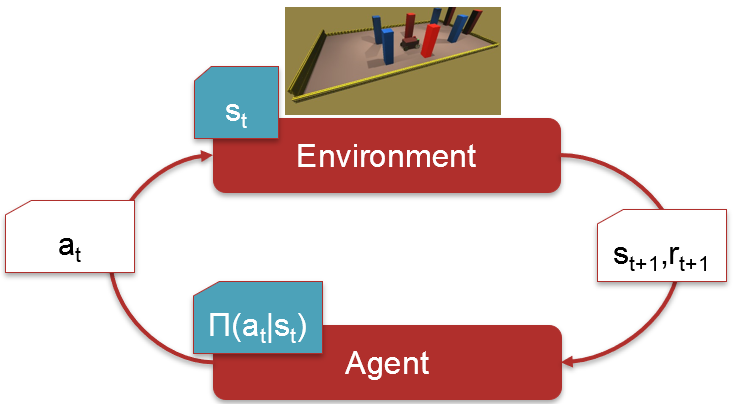
\includegraphics[width=0.8\textwidth]{Bilder/rl_cycle.png}
%    \caption{Loop in Collect Data}
%    \label{fig:unitycommunication}
%\end{figure} % TODO can we use this image?

Recent avancements in artificial intelligence technology have made it possible to develop automated solutons for a wide range of tasks that were previously thought to be too complex and unfit for machines to solve. Most notably over the last few years is the introduction of diffusion image models and large language models. These technologies were well recieved and moved artificial intelligence tools into public discourse. All over the world people have recognized the potential of artificial intelligence technologies and are now using them in their daily life and at work.

Artificial intelligence has already been of big importance in academia and industry for a long time. AI has been proved useful in many different fields, such as image recognition, natural language processing, and robotics. This encourages researchers and industry to further develop and use AI in their work. A promissing domain for the application of AI is autonomous driving.

The development of autonomous vehicles promises to greatly reduce the number of traffic accidents and transportation cost \autocite{mckinsey}. The development of autonomous driving could have further downstream effects on our society and industry, such as for example improved logistic and transportation systems.
As a result, researchers and private enterprises from all over the globe are making progress towards fully autonomous driving agents. Many companies started to integrate adaptive cruise control and lane centering assistance \autocite{carreviews} in their products. Due to the recent developments in artificial intelligence and the very high complexity of the task of autonomous driving, artificial intelligence often plays a big role in these systems \autocite{drl_for_ad}.

Predictions for the future of autonomous driving have been very optimistic and although huge progress has been made, the task of fully autonomous driving is still far from being solved \autocite{state_of_autonomous_driving2023}. This thesis aims at contributing to the research in this field by applying reinforcement learning to autonomous driving agents in a simulated environment. This work builds upon the work of \autocite{maximilian} and will use the same task and evaluation metrics. This thesis focusses on improving the agent's resiliency to changing light conditions by training a convolutional neural network end-to-end using reinforcement learning.


\chapter{Research Goals}
\label{cha:ResearchGoals}

The goal of this thesis is to contribute in the domain of autonomous driving by investigating the use of \ac{RL} to train an autonomous driving agent that is resilient to changes in light conditions. The agent is evaluated on simulated tracks that consist of a series of goals indicated by two blocks, a tracks is successfully completed if the agents drives through all goals in order \ref{fig:track_and_agent}.
This thesis builds upon previous work at the ScaDS.AI \textcite{maximilian} and uses the same tracks and task specifications. The agent from previous work was not able to reliably complete tracks under changing light conditions, motivating the research goals.


The agent and the policy are designed to be resilient to light changes. To achieve this, the policy is trained using \ac{RL} in a simulated environment with changing light conditions. The policy consists of a \ac{CNN}, the inputs to the \ac{CNN} are camera images from the perspective of the agent \ref{fig:track_and_agent}. Preprocessing steps are applied to the camera images to improve the performance of the policy under changing light conditions. The policy is trained end-to-end using an \ac{RL} algorithm. This allows the policy to learn the relevant features from the camera images itself.
Different training approaches and preprocessing steps to develop a powerful agent are investigated.


\begin{figure}
    \centering
    \subfigure{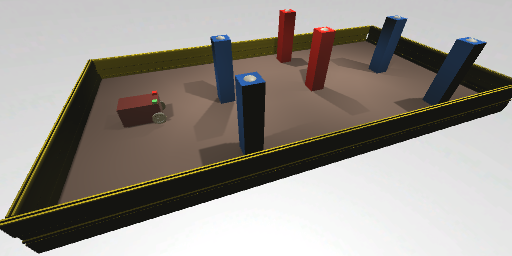
\includegraphics[width=0.4\textwidth]{Bilder/image_printer_images/evaluation_hard.png}}\qquad
    \subfigure{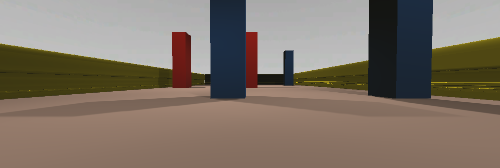
\includegraphics[width=0.4\textwidth]{Bilder/image_printer_images/agent_image_from_unity.png}}\\
    \caption{Example image of a track and the agent's camera}
    \label{fig:track_and_agent}
\end{figure}


\section{Question 1 - \questionOne}

The previous work by \textcite{maximilian} showed that it is possible to train an agent using \ac{RL} to solve the evaluation tracks, however the trained agents were not successful in reliably traversing the tracks of higher difficulty levels. The agents developed in previous work utilized an extensive preprocessing pipeline to extract the relevant information from the camera images for processing by the policy. The evaulation by \textcite{merlin_flach} showed that the preprocessing pipeline's performance depends heavily on the light settings of the environment.

This thesis will use a \ac{CNN} network policy that is trained end-to-end using \ac{RL}. It has already been shown to be possible to train an agent to solve the autnomous driving task using \ac{RL}. However the agents developed in previous work used different preprocessing steps and policies compared to the agents developed here.

Due to these differences in implementation and as a prerequisite for question 2 and 3, it is first important to investigate if it is possible to train a \ac{CNN} policy to reliably solve the tracks of all difficulty levels. This raises question 1:
\questionOne

The question will be answered by developing agents based on related work. The training process of the agents will use common practices from \ac{RL} adapted to the specific task. The developed agent's $success\_rate$ and $collision\_rate$ will be evaluated on all difficulty settings to answer the question.


\section{Question 2 - \questionTwo}

Question 1 investigates if it is possible to develop a successful \ac{CNN}-based agent solving the tracks of all difficulty levels. 
Question 2 then investigates if it is possible to make the \ac{CNN}-based agents robust to changing light conditions.

The agents developed for question 1 will be used as a basis for the agents developed in this question. The agents will be augmented with preprocessing steps that improve the performance of the agents under changing light conditions. These preprocessing steps will be applied to the camera images before they are processed by the policy. The agent's policy will be trained in a simulated environment with changing light conditions to help the agent generalize and learn.

Similarly the $success\_rate$ and $collision\_rate$ will be primarily used to evaluate and compare the agent's performance. The performance difference between different light conditions will be used to answer the question. If the performance for all light conditions is comparable to the performance of agents in question 1, the agents can be considered robust to changing light conditions.

\section{Question 3 - \questionThree}

One goal of the ongoing research at the ScaDS.AI is to build physical robots for demonstration and research purposes \textcite{merlin_flach}. The robots are based on the NVIDIA JetBot platform \autocite{jetbot}. They are equiped with a camera, wheels and a small on-board computer. A future goal is to transfer trained policies onto these robots and execute them in real-life. However the limited processing power of these robots might not be sufficient for more complex agents that utilize \acp{NN}. This raises question 3 - \questionThree


The question will be answered by investigating the processing power required to run the preprocessing steps and \acp{NN} used in the agents. This will be evaluated empirically by creating recordings of the agents in simulations. The recordings are then replayed on the physical hardware. The evaluation checks if the physical hardware is able to reproduce the preprocessing steps and policy from the replays in real-time.



\chapter{Related Work}
\label{cha:Related Work}


The development of self-driving cars represents one of the most intricate and ambitious challenges in the field of engineering, robotics and artificial intelligence. The complexity and variability of real-world driving environments make this task extremely difficult. The environments include unpredictable actors, such as other drivers, pedestrians, and animals, as well as changing weather and road conditions. The environments include uncounted edge cases that are difficult to anticipate and code for explicitly. Consequently, many researchers and institutions include advanced machine learning techniques in their approaches towards solving autonomous driving.

The development of autonomous driving systems started with driver assistance systems in the 1970s. These systems focus on assisting the driver in specific tasks, such as lane keeping, adaptive cruise control, and parking. This reduces the problem complexity. However modern self-driving systems aim to achieve full autonomy. For example the Tesla autopilot is capable of driving in many environments without human intervention.

This thesis will use reinforcement learning in the training of an autonomous driving agent. The agent is equiped with a single camera sensor. The agent's behaviour is controlled by a convolutional neural network that processes the visual input. The agent has to learn a specific self driving task with reduced complexity. The self-driving task is similar to previous research at the ScaDS.AI \textcite{maximilian}. However the agent design and training is very different.
The task consists of a restricted environment. The environment consists of an enclosed arena with different tracks that the agent has to complete. The tracks consist of a series of goals that the agent has to drive through. The tracks are grouped in three difficulty levels.
The environment is simulated with three light settings. The trained agent has to learn to navigate all difficulty levels and light settings.

Research relating to reinforcement learning algorithms, convolutional neural networks and self-driving will be reviewed.
% also research regarding rebustness to light changes?

% TODO auch die Ergebnisse der Paper und die daraus gezogenenn Schlüsselideen erwähnen


\section{Self-Driving}

Neural networks have been used in the domain of self driving for a long time. Pomerleau \textcite{alvinn} developed one for the first self driving systems with neural networks in 1989. The system was developed for road following. The system used a camera image and a laser range finder as input. Compared to current network sizes, they used a small fully connected neural network. The network was trained using synthetic data. The data consisted of generated road images and steering commands. The network was trained using backpropagation to reproduce the steering commands. This approach did not use reinforcement learning. The system was able to follow roads in real-life under certain conditions.
The paper highlights the advantages of neural networks for self-driving. The training data determines the salient image features and not the programmer. This has proven to be true with the success of convolutional neural networks in the domain of self-driving \textcite{neptune}.


There has been a lot of progress in the domain of self-driving in recent years. Sophisticated self-driving algorithms consist of many hardware and software components to achieve satisfying performance. Hardware components include various imaging approches such as Radar, Lidar and cameras. Termometers and other hardware components are also used, for example to determine weather conditions. 
Software components might include separate object detection, occupancy and planning. For example Tesla's self-driving builds these components on top of a shared backbone that uses convolutional neural networks \textcite{howteslaautopilot}.
% (CNN is ResNet)

Self-driving in a real world environment is a very complex task, especially when including other traffic participants. Modern self driving agents consist of multiple complex components that interact with each other \textcite{drl_for_ad}. Components for Scene Understanding build a model of the current surroundings. The Descision making \& Planning components use this model to decide and execute the next actions.
Multiple interacting components are shown in figure \ref{fig:ad_components}.

\begin{figure}
    \centering
    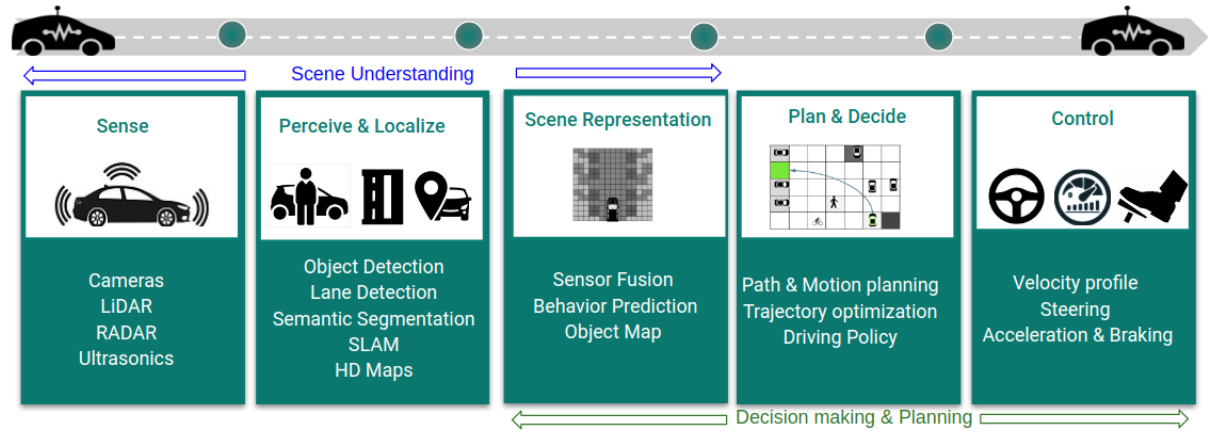
\includegraphics[width=0.8\textwidth]{Bilder/ad_components_from_paper_drl_for_ad.png}
    \caption{Standard components in a modern autonomous driving systems pipeline listing the various tasks. The key problems addressed by these modules are Scene Understanding, Decision and Planning. Image from \textcite{drl_for_ad}}
    \label{fig:ad_components}
\end{figure}

An agent with similarly complex components is not feasible for this thesis. The agent in this thesis uses a single convolutional neural network to process the visual input and make decisions instead. I aim to contribute to the domain by expanding on previous research and focus on the training of a convolutional neural network agent. 


TODO wohin diesen satz?
Approaches from the domain of self-driving will be used to improve the training of the agent, for example reward shaping \textcite{drl_for_ad}.

\subsection{Previous Work}
This thesis builds directly upon the work of Knig \textcite{jonas_koenig}, Flach \textcite{merlin_flach} and Schaller \textcite{maximilian}. 
\textcite{jonas_koenig} built a self-driving agent that was trained to avoid collisions in a simulated arena. The agent used a hand-crafted preprocessing pipeline to extract features from visual input. The features represent the obstacles that the agent has to avoid. The agent's behaviour was controlled by a policy that consisted of a neural network. This network used the extracted features as inputs. It was trained using an evolutionary approach in simulation.

\textcite{merlin_flach} investigated the feasibility of transferring this agent to the real world. The research showcased many challenges. The challenges are caused by differences between the simulated and real-life environments, the Simulation-To-Reality gap. The most notable problem was the object recognition part. The preprocessing pipeline had difficulties recognizing the objects in the real world. This results in further problems for the agent, since the agent's policy is based on the extracted features.

\textcite{maximilian} investigated a different task than the two previous papers. An agent was trained to traverse a track by driving through a sequence of goals. The same tracks are used in this paper. The agent used a preprocessing pipeline to extract object features similar to \textcite{jonas_koenig}. The neural network policy was trained using the proximal policy optimization \textcite{ppo} reinforcement learning algorithm. The agent could traverse the tracks, its performance decreased for tracks of higher difficulty. Further evaluation of the agent under different light settings showed that the agent is not robust to changing light conditions. The preprocessing pipeline was not able to extract the necessary features reliably under different light settings, this resulted in a performance collapse.

The instability of the hand-crafted preprocessing pipeline and promissing results by CNNs from other RL researchers in the domain of self-driving \textcite{neptune} motivate the choice of CNNs as the feature extraction method in this thesis. 


\section{Reinforcement Learning}

% data not programmer decides the salient image pixels (bedeutungsvollen)
\subsection{Introduction to Reinforcement Learning}

Reinforcement Learning algorithms have been around for a long time, but only recently have they been able to achieve superhuman performance in games and control tasks \textcite{atari}. Reinforcement learning algorithms formalize the problem as consisting of an environment and a policy $\pi$. The environment consists of a state space, an action space and a reward function that takes state-action pairs as input. Reward functions assign positive rewards to actions that are deemed to be desirable by the environment designers, for example scoring a goal in a football match. Reward function can also assign negative rewards to undesirable actions, for example collisions in a driving simulation. 

The goal of reinforcement learning algorithms is to build an agent that interacts with its environment and maximizes the cumulative reward over time. The policy selects actions given an observation. It controls the agents behaviour \textcite{rlbook2020}. It is trained by the \acs{RL} algorithm to learn the desired behaviour. The trained policy can then be used to solve problems in the environment. 

The agent interacts with the environment during the training phase of RL algorithms. The policy takes some representation of the environment's state as input and selects actions to execute in the environment. The selected actions are executed in the environment by the agent which results in a new state. The reward function assigns rewards to these state transitions.
The observed rewards are then used to update the policy \ref{fig:rlcycle}.

\begin{figure}
    \centering
    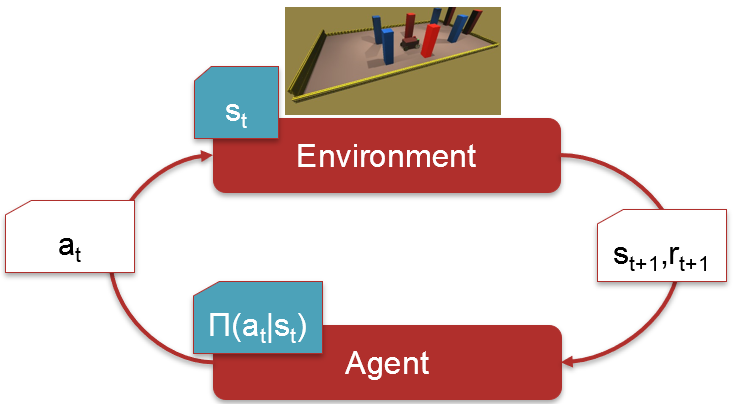
\includegraphics[width=0.4\textwidth]{Bilder/rl_cycle.png}
    \caption{RL Training Cycle: The agent selects action $a_t$ based on policy $\pi(a_t|s_t)$ at state $s_t$ and recieves the next state $s_{t+1}$ and rewards $r_{t+1}$ from the environment. The states, actions and observed rewards are used to update the policy.}
    \label{fig:rlcycle}
\end{figure}

\subsection{Classification of \acs{RL} Algorithms}

Reinforcement learning algorithms are classified into two major groups. RL algorithms that use a model of the environment are called model-based algorithms, algorithms without such models are called model-free algorithms. Algorithms from both groups have been successfully used in a wide range of applications, model-based algorithms are often much more complex but have been shown to be successful at many task that require planning \textcite{alphagoimprovementmuzero}. Model-free approaches are often simpler and more flexible, they have shown great success in various control tasks \textcite{atari}.

\begin{figure}
    \centering
    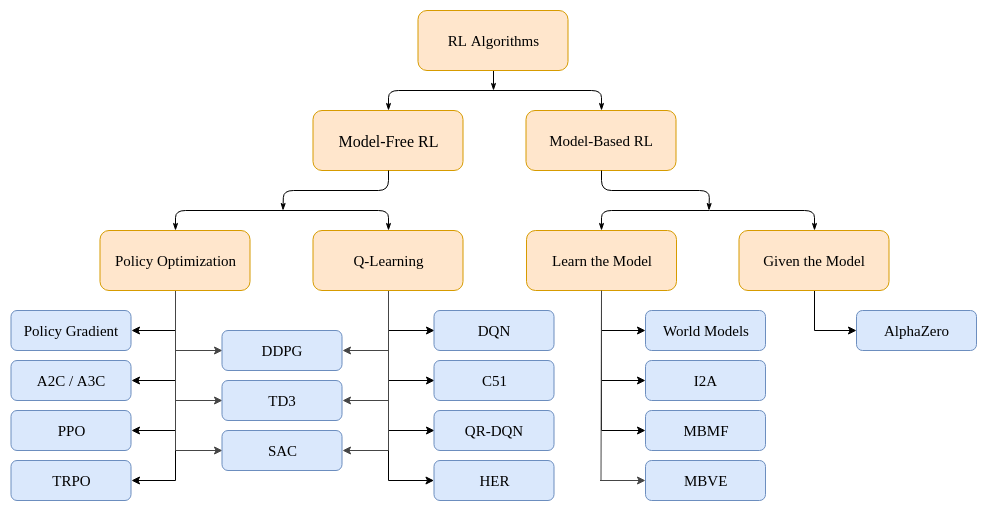
\includegraphics[width=0.8\textwidth]{Bilder/openai_spinningup_taxonomy.png}
    \caption{Taxonomy of RL algorithms from OpenAI's Spinning Up course \autocite{spinningup}}
\end{figure}

\subsubsection{Model free \acs{RL} Algorithms}

\paragraph{Value based algorithms}
Model free algorithms can be further divided into two families. The first family are value-based approaches. These algorithms learn a function that assigns state-action pairs a value. This function is called the value function. This value represents the expected future reward Q.
 
The policy is not trained directly. The policy selects actions based on this value function instead. The state-action pair with the highest Q-value is selected for a given state.

The training process of the value function is done by updating the Q-values based on the observed rewards. The Q-learning algorithm is an early and common example of value-based algorithms \textcite{rlbook2020}. The Q-learning algorithm updates the values based on the observed rewards and the maximum Q-value of the next state \[Q(S_t, A_t) = Q(S_t, A_t) + \alpha (R_{t+1} + \gamma \max_a Q(S_{t+1}, a) - Q(S_t, A_t))\].
$\alpha$ is the learning rate. It determines how quick values are changed. $\gamma$ is the discount factor of future rewards.


The Q-learning algorithm can use a table to store the value function. The table contains one cell for each state-action pair and stores the Q-value. 
For many problems the use of these tables in not feasible due to the amount of state-action pairs, many extensions to the algorithms have been developed such as for example deep q-learning. Deep q-learning uses a deep neural network to approximate the Q-values \textcite{atari}. The network learns to predict the Q-values for state-action pairs. Neural networks are general approximators. They can learn to generalize and return accurate value predictions even for previously unseen states.  

Value-based \acs{RL} algorithms have been used to great success for control tasks \textcite{rlbook2020}. However they will not be used in this thesis, as they require discrete action spaces. The environment in this thesis consists of a continuous action space.
An action space can be discretized for use by value-based algorithms \ref{fig:example_discretization}. However this can lead to a loss of fidelity.

% TODO \ref{fig:example_discretization} ?

\paragraph{Policy based algorithms}
% rlbook2020 chapter 13.7
The other family are policy-based algorithms. These algorithms optimize the policy directly instead of the values associated with states or state-action pairs. Instead of computing the learned probability of each action, the policy learns the statistics of the action distribution.
Given a scalar action space. The action distribution can be represented as a gaussian probability Distribution:
\[p(x) = \frac{1}{\sqrt{2\pi\sigma^2}} e^{-\frac{(x-\mu)^2}{2\sigma^2}}\]

The policy can then be defined as the normal probability density over a real-valued scalar action. The mean and standard deviation of the distribution are given by parametric function approximators that depend on the state $s$. The mean is given by $\mu(s, \theta)$ and the standard deviation by $\sigma(s, \theta)$. The policy is then defined as:
\[\pi(a|s, \theta) = \frac{1}{\sigma(s, \theta)\sqrt{2\pi}} e^{-\frac{(a-\mu(s, \theta))^2}{2\sigma(s,\theta)^2}}\]

The parametric function approximators $\mu(s, \theta)$ and $\sigma(s, \theta)$ are trained by the \acs{RL} algorithm. Any function approximator can be used, for example a \acs{NN} with parameters $\mu$ \textcite{rlbook2020}. 

The action distribution can be extended to multi-dimensional action spaces. This action distribution can be represented as a multivariate gaussian distribution. The function approximator then outputs the mean and covariance matrix of the distribution. This makes policy-based \acs{RL} algorithms very flexible. They can be used for multi-dimensional continuous action spaces.


The policy can be updated using the gradient of the expected rewards with respect to the policy parameters. Algorithms that use this approach are called policy gradient algorithms.


\paragraph{Actor-Critic Algorithms}
Alternatively the policy can be updated using Actor-Critic approaches. These combine policy-based and value-based approaches. Actor-Critic approaches contain a policy and a value function. The value function represents the expected future reward of a state. The policy is updated using this value function.

The Proximal Policy Optimization algorithm is an Actor-Critic algorithm. It was developed to improve the stability of policy-based algorithms \textcite{ppo}. The \acs{PPO} algorithm restricts the size of policy changes caused by parameter updates, which ensures the policy does not change drastically. This improves stability. \acs{PPO} is currently one of the most popular algorithms for reinforcement learning. It has already been successfully used in the domain of autonomous driving \textcite{maximilian}.



% Another major improvement in the domain of reinforcement learning was the combination of neural networks with traditional planning and search algorithms, the most famous example for this is AlphaGo \textcite{alphago}. These algorithms often are model-based algorithms and use search algorithms (e.g. Monte Carlo Tree Search)  to evaluate the possible actions at a given state. The neural networks are used for the evaluation of states and actions in the search algorithms. AlphaGo was developed for a 2 player deterministic game with a discrete state and action space. Since then this combination of neural networks and search algorithms has also been used to achieve impressive results for all kinds of problems \textcite{alphafold}, for example single player continuous state and action spaces \textcite{alphagoimprovementmuzero}. Although these algorithms could be applied to the problem at hand, they will not be utilized due to the increased complexity of the algorithms and the required computational resources.
% TODO sollte der Teil wieder rein?

% temporal difference learnign: update a function based on previously learned things (e.g. q-learning)

% TODO mention reward shaping from rlbook somewhere
% first give a reward signal that is not aligned with final goal but gives frequent rewards
% train the agent using this function
% change function over time to the intended reward function (event Reward)
% learning behaviour is guided by the shaped reward function



\subsection*{Convolutional Neural Network for Reinforcement Learning}

Convolutional neural networks are a neural network architecture specifically developed for processing image data, they consist of a number of filters and a fully connected neural network. The filters are applied to the image in a sliding window fashion, the filters detect patterns in the image such as for example edges and corners. Multiple successive applications of such filters enables the network to learn hierarchical information and recognize more complex structures. The fully connected neural network analyses the results of the filters and makes the final prediction \textcite{rlbook2020}.

CNNs are often used in Reinforcement Learning since RL problems often require an agent to process visual input. Furthermore CNNs can be trained end-to-end in Reinforcement Learning compared to other feature extraction methods, which means the CNN can learn what features are important for the task at hand.
Therefore a convolutional neural network will be used to process the camera images instead of a hand-crafted feature extraction method. 

CNNs typically do not take the raw camera/simulation images but rather preprocessed images, e.g. greyscaled images \textcite{atari}. Preprocessing steps can help in reducing the complexity of the input space. Convolutional neural networks require a lot of data to train, data augmentation can help increase the size of the training set and to make the agent more robust. Data augmentation generates new samples from already collected ones by applying transformations to the samples. 


% TODO move next paragraph to CNN section?
The PPO algorithm can be used to train agents that use convolutional neural networks as their policy. Convolutional neural networks are ideal for processing image data and can be trained end-to-end by the algorithm \textcite{ppo}. 

% rlbook2020 chapter 9.7 explains the use of CNNs in RL



% \textcite{autonomous_vehicles_review} %TODO read this paper and cite it

% https://safe-intelligence.fraunhofer.de/en/autonomous-driving

% Papers that use Carla



\section{Simulation for Reinforcement Learning and Self-Driving}

% TODO Carla und andere Simulations machen keinen Sinn, da wir ein festse Problem haben

Simulations play a huge role in reinforcement learning and thus the development of self-driving agents. Simulations provide a huge number of benefits over real world experiments. They are much cheaper and faster to run than real world experiments, furthermore they can be run in parallel. In addition the programmers have direct and perfect control over the environment, as such programmers can for example change the simulation speed. This allows for fast experimentation and training of reinforcement learning agents. Simulations also allow for the creation of scenarios that are not possible in the real world. This is especially useful for reinforcement learning agents that are trained to avoid collisions. Simulations also allow for the creation of ground truths such as perfect sensor data and object bounding boxes \textcite{carla}.

Simulated environments often serve as baselines for reinforcement learning algorithms, most famous are the atari games \textcite{atari}. The Python Gynasium API was developed for easy reuse and comparison of reinforcement learning algorithms for different problems \textcite{gymnasium}, the Gymnasium API defines an interface that can be used to model tasks as reinforcement learning problems. A wide range of reinforcement learning frameworks support the Gymnasium API, for example Google's dopamine \textcite{dopamine} and OpenAI's baselines \textcite{sb3}. Advanced simulations like the Unity engine \textcite{unity}, the physics simulator MuJoCo \textcite{mujoco} and the driving simulator Carla \textcite{carla} can be integrated with the Gymnasium API.

%The complexity and interest in self-driving has also led to the development of dedicated simulators, such as the Carla \textcite{carla} and the AirSim \textcite{airsim} simulator. The Carla simulator provides researchers with useful features such as weather control and ground truths for object detection and segmentation.

There are also dedicated frameworks for reinforcement learning that directly integrate with simulation engines. \textcite{maximilian} used the ML-Agents framework \textcite{mlagents} to train the self-driving agent in Unity directly.

In this thesis Unity will be used for the simulation, the simulation will be integrated with the Python Gymnasium API and PPO algorithm. This approach is chosen instead of the ML-Agents framework since it allows for more flexibility and control over the simulation and training process.


\section{Imitation learning}
As described before it is difficult to build self-driving agents for real world environments due to the environment complexity. The amount of complex edge cases make it very difficult to programmatically define the agent's behaviour. Neural networks can be used to control the agent behaviour instead. The neural networks can be trained using reinforcement learning in simulation. 
Imitation learning is another approach to training an agent that interacts with its environment. Imitation learning requires a dataset that demonstrates the desired behaviour. The agent is trained on the dataset to mimic the expert behaviour.

In reinforcement learning the programmer has to define a reward function that the agent uses to learn and improve its behaviour. In imitation learning the agent learns exclusively from the dataset. As a result this dataset has to include a wide range of scenarios to produce a reliable agent that can handle edge cases.

There are two approaches to training an agent with imitation learning, behavioural cloning and inverse reinforcement learning. Behavioural cloning is the simpler approach, the agent learns to mimic the expert behaviour directly. This is similar to supervised learning. Inverse reinforcement learning is more complex, the reward function from the expert demonstrations is learned first. The agent is then trained to maximize this reward function using reinforcement learning. 

Bojarski \textcite{bojarski2016endToEnd} used imitation learning to train a self-driving lane following agent for real-world environments. This agent consists of a convolutional neural network that processes the camera images and predicts the steering angle directly. The agent is trained end-to-end to reproduce steering behaviour from recorded data. They demonstrate that imitation learning is a viable approach for developing an agent without the need for multiple components such as object detection and path planning.

Tesla used imitation learning to train the path prediction component of their self-driving systems. The fleet of Tesla vehicles allows them to collect a large amount of representative data in the real world. The reference dataset was generated from recordings of human Tesla drivers \textcite{tesla_youtube}. 

Imitation learning and reinforcement learning can be combined to improve the training of the agent. The reinforcement learning process generates samples via interaction between agent and environment. These samples and the expert behaviour dataset are used together to train the agent policy \textcite{car-following_carla_dresden}.


%\section{Reinforcement Learning for Self-Driving}

%\textcite{drl_for_ad} review the use of reinforcement learning for autonomous driving, they also describe many improvements for reinforcement learning algorithms that can improve the training stability and performance, such as for example reward shaping.
%In addition to published research papers there have been a lot of experiments, tutorials and demonstrations of self-driving agents on YouTube and GitHub. The University of Tübingen published their full lecture series on Self-Driving Cars \textcite{tuebingen}, the series also includes a section on reinforcement learning.

% papers that cite carla: https://scholar.google.de/scholar?cites=660591080772510291&as_sdt=2005&sciodt=0,5&hl=de


% Tübingen: % https://www.youtube.com/watch?v=GYnlqiSqZiU&list=PL05umP7R6ij321zzKXK6XCQXAaaYjQbzr&index=13



% Key Papers in RL: https://spinningup.openai.com

\section{Light change resiliency}

\subsection{Domain Randomization}

useful for transfer sim-to-real
https://ar5iv.labs.arxiv.org/html/1703.06907

domain randomization for sim-to-real tries to teach the agent to solve a task under a big variety of conditions in simulation, the hope is that the agent will be able to generalize this variation and learn in this environment.
The real world is simply one variety that the agent might have already learned to generalize.

The randomization can include textures, image resolutions, ..., motor power of agent in sim, ... (physical properties)


domain randomization can lead to a high variance of policy performance for different environment randomizations. The paper https://ar5iv.labs.arxiv.org/html/1910.10537 introduces a regularization approach for the policies.
visual vs dynamics randomization (camera changes vs physics e.g. friction of wheels)

\subsection{Data augmentation}

Data is collected in simulation and then augmented


\subsection{Multi-Modal learning}

Provide the agent with more than just image data,  e.g. radar...


\subsection{Hierarchical Reinforcement Learning}

combination of multiple levels. higher level policy controlls the actions, the lower level policy learns to build representations for the higher level policy

Hierarchical Reinforcement Learning: Using a hierarchical approach where high-level policies govern low-level policies can help the agent adapt to changing conditions more effectively. High-level policies can decide on strategies based on the overall environment, while low-level policies handle specific tasks like adjusting to lighting changes


TODO relate the previous work that used a hand-crafted feature extraction pipeline to hierarchical rl

\section{Transfer to reality}

\subsection{Transfer Learning}
learn on diverse data and then fine-tune on real data


\section{Key Ideas}

\subsection{Fitting RL algorithms}

\subsubsection{CNN for feature extraction in RL}

\subsubsection{Memory mechanism}


\subsection{Reward shaping}

\subsection{Environment Implementation}

speed of environment is critical...


\subsection{Image preprocessing for resiliency to light changes}

\subsection{Domain Randomization}






\chapter{Methods}
\label{cha:Methods}



\section{Task Description}

In this section I will be describing the task and the simulation environment as these two aspects are the foundation of this thesis and will not change over the course of the project.
The task is to develop an agent using reinforcement learning that is able to complete a parcour in a simulated environment without collisions. The agent has to traverse the parcour by passing through a number of goals indicated by pairs of either red or blue blocks without collisions. This problem belongs to the class of single player continuous state and action space problems. At each timestep the agent uses a neural network to process an image from the environment and produce two actions. The two actions are the acceleration values of the left and right wheel, these acceleration values are applied to the wheels until a new action is selected.% The timesteps do not have a fixed duration, a new timestep is started as soon as the last one is finished. The amount of timesteps per minute will be measured? This is like FPS?

The task and agent are simulated using the Unity game engine, the game engine handles the rendering of the environment, collisions, agent movement and reward functions.


\begin{figure}
     \centering
     \subfigure[Example image of the agent at the start of a parcour with 3 goals in Unity]{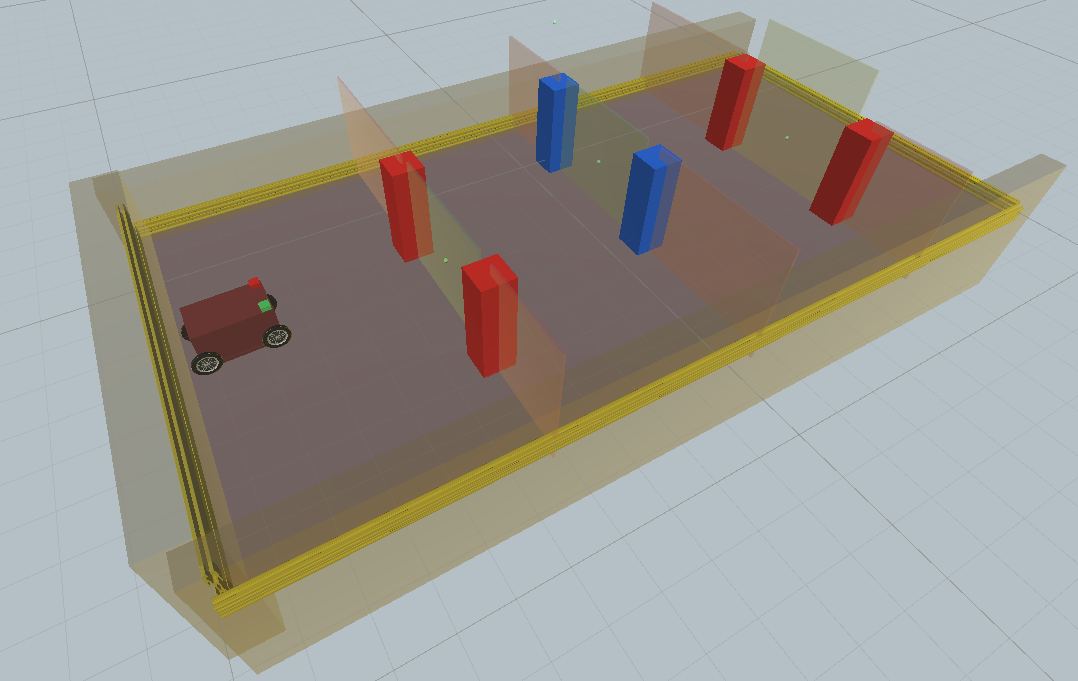
\includegraphics[height=5cm]{Bilder/parcour.png}}\qquad
     \subfigure[Agent camera view]{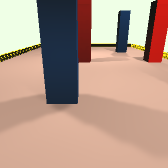
\includegraphics{Bilder/agent_input_image2.png}}\\
     \caption{Unity simulation environment and agent camera view}
\end{figure}


\iffalse
     \begin{figure}[h!]
          \centering
          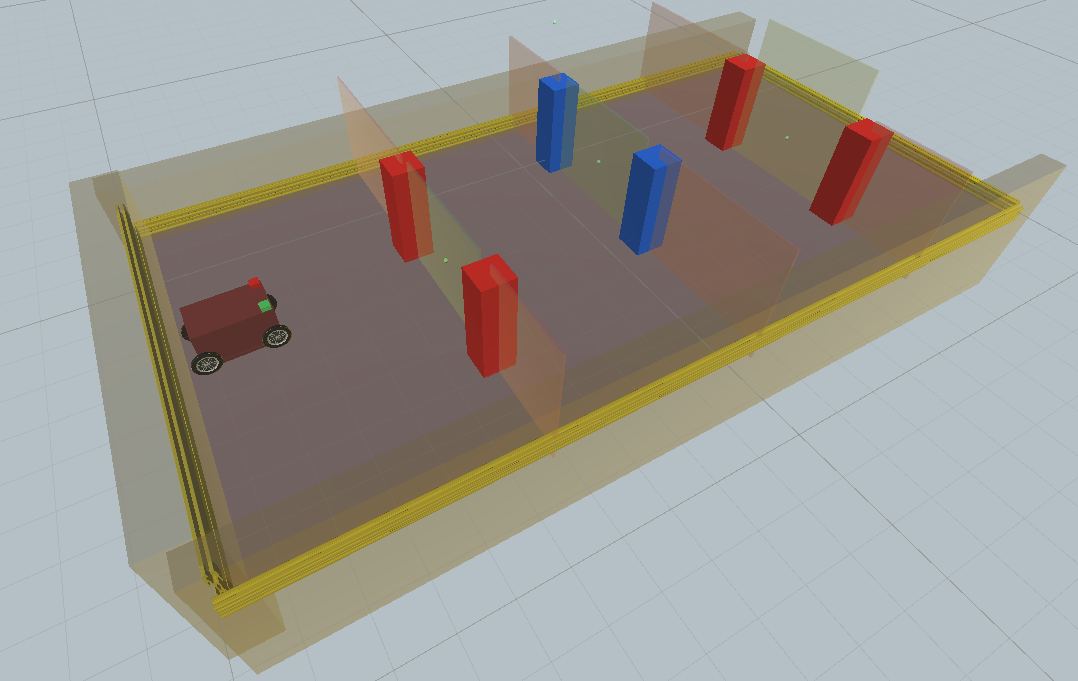
\includegraphics[height=7cm]{Bilder/parcour.png}\\[2.5ex]
          \caption{Example image of the agent at the start of a parcour with 3 goals in Unity}
          \label{task}
     \end{figure}
     \begin{figure}[h!]
          \centering
          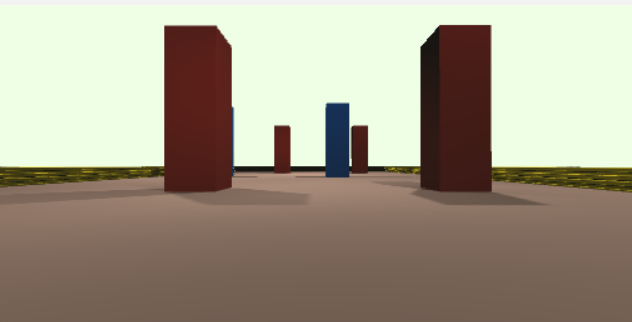
\includegraphics[height=7cm]{Bilder/agent_input_image.png}\\[2.5ex]
          \caption{Example image that will be processed by the agent's convolution neural network.}
          \label{input_image}
     \end{figure}
\fi

% mention the similarity/simplicity of the task


\section{Reinforcement learning algorithm and frameworks}

As outlined in the related works section many different RL algorithms can be used to solve single player continuous state and action space problems. The PPO algorithms is most commonly used for problems of this class and has already been successfully used in the investigated task \autocite{maximilian}. The MuZero \autocite{alphagoimprovementmuzero} could also be used, however this algorithm does require a lot more compute resources during training and inference.
In this thesis the PPO algorithm will be used.

There are multiple approaches to training an agent in the Unity simulation environment as highlighted in the related works section, it is not yet decided which approach will be chosen, therefore I will quickly describe the possible scenarios and highlight their advantages and disavdantages.

\subsection*{Unity and ML-Agents}

Reinforcement learning agents can be trained directly in the Unity simulation environment using the ML-Agents framework \autocite{mlagents}. This approach has the advantage of being very simple to implement and use, since the agent and simulation are in the same framework. The biggest disadvantage of this approach is that it might be difficult to implement some of the implementation details that might be used in this thesis such as the proposed changes for dealing with delayed rewards.
The PPO algorithm by \autocite{mlagents} was used in \autocite{maximilian} to successfully train the agent on the investigated task.

\subsection*{Unity and separate reinforcement learning frameworks}

There are many reinforcement learning frameworks publicly available that can be used to train agents in simulated environments, such as the OpenAI's baselines \autocite{sb3} and Google's dopamine \autocite{dopamine}. These frameworks often support the Gymnasium API \autocite{gymnasium}, wrapping the Unity simulation environment in a Gymnasium environment would allow for easy use of these frameworks. This approach has the advantage of being able to use the many features of these frameworks and makes it easy to change the training algorithms which might be necessary for the investigated implementation details. The disadvantage of this approach is that it might be difficult to wrap the Unity simulation environment in a Gymnasium environment, there already exist frameworks to help with this \autocite{peacefulpie}.


% maybe mention the similarity/simplicity of the task here to show PPO is good


\section{Investigated implementation details}

The goal of this thesis is to answer two questions with a subitem each.
\begin{enumerate}
     \item Is it possible to train an agent to reliably solve the parcours of all difficulty levels?
           \begin{itemize}
                \item Are memory mechanisms necessary in achieving this?
           \end{itemize}
     \item Is it possible to use an end-to-end trained CNN to make the agent robust to changing light conditions?
           \begin{itemize}
                \item Is it possible to use a CNN which is small enough to be used in the JetBot?
           \end{itemize}
\end{enumerate}

\subsection{Improvements for training the agent}

\subsubsection{Reward shaping}

Reward shaping is the practise of providing reinforcement learning agents with frequent and accurate rewards. This helps the agent develop the desired behaviour quicker and more reliably since reward signals are less sparse with reward shaping \autocite{drl_for_ad}. This practice was already employed by \autocite{maximilian} by providing the agent with a reward proportional to its speed, this encourages the agent to drive faster and thus hopefully complete the parcour quicker. This thesis will investigate the use of a reward proportional to the difference in distance to the next goal between timesteps, this should encourage the agent to drive towards the next goal and to drive faster in this direction.


\subsubsection{Dealing with delayed rewards}
Delayed rewards can be a big problem in reinforcement learning and make the training process difficult. Delayed rewards are rewards that are not obtained immediately after the responsible action is taken. In our environment an action \(a_n\) (e.g. turning right) may lead to a collision at state \(s_{n+x}\) which results in a negative reward for action \(a_{n+x}\). The RL algorithm might fail learn to avoid the action \(a_n\).

There are a multiple approaches to dealing with delayed rewards. These approaches use the reward at the current timestep and the near future. These approaches result in a more accurate and dense reward signal and can improve the training stability and performance of the agent.
N-step bootstrapping uses the rewards at the current step and the next \(n\) steps \autocite{nstepbootstrapping}.
A similar approach does not use the reward from the next \(n\) steps but rather the cumulative reward encountered in the next \(n\) seconds \autocite{trackmania}. Due to the continuous nature of the environment this approach might be more suitable than the previous one.


\subsubsection{Time perception}

Two configurations of the agent by \autocite{maximilian} used a memory to enhance the agent's input, the memory consisted of the input of the last few steps of the agent. This technique of stacking the history has been widely used in RL for continuous \autocite{atari} and discrete action spaces \autocite{alphago}. This allows the agent to perceive object movement, time and velocities \autocite{atari}.
In our case the agent needs a history since the next goal could leave the agent's current field of vision.

%However since the investigated environment does not have fixed timesteps this approach might not be as effective. The time elapsed between two steps can vary due to many factors such as varying compute resources. It could prove useful to provide the model with the input of the last few steps and in addition the elapsed time between these steps. % these few sentences only make sense if the varying time is dicussed in the first part of the Methods section

% TODO test other memory mechanisms?
% like for example also feeding the previous time step's hidden layer activation as input
% that way the agent would know the previous "decision" not just the previous input

\subsection{Improvements for Light setting robustness} \label{light_setting_robustness}

\subsubsection{Convolutional Neural Networks}

The works by \autocite{merlin_flach} and \autocite{maximilian} showed that the agent's performance greatly depended on the quality of the input preprocessing pipeline. This object detection pipeline had difficulties detecting objects under varying light settings. This thesis will investigate using convolutional neural networks instead of an object detection pipeline, this should make the agent more robust to varying light settings and improve the performance of the agent.
Using convolutional networks to process images is a common practise in the field of reinforcement learning, due to the ability of these networks to adapt. The convolutional neural network could potentially learn to identify relevant information in images more reliably than the previously used image detection pipeline. The research by \autocite{merlin_flach} showed that not all the information provided by the object detection pipeline was considered to be relevant by the neural network, this could be mitigated by training the CNN end-to-end.
As a starting point for experimentation the CNN architecture will be the same as \autocite{human_level_control}.

% we use the default CnnPolicy network, is it the same as the one described in Atari?
% architecture: https://github.com/DLR-RM/stable-baselines3/blob/d671402c9373391f44d8a2ad11deed615e0f4bae/stable_baselines3/common/torch_layers.py#L89-L106
% it is exactly as described in "Human-level control through deep reinforcement learning"
% \autocite{atari} has a slightly smaller NN

% (more robustness?) (previous input was shit (sim2real paper wegen x, y, width, height input problem)) (previous system higly depended on bounding box detection)


\subsubsection{Feature reduction / preprocessing}

There are several preprocessing approaches that can be used to prepare an image for processing by a convolutional network. The goal of these approaches is to reduce the feature space to increase processing speed, they can also help encourage the network to generalize. The following steps were taken in the foundational \autocite{atari} paper. These techniques will be used due to the similar complexity of our task and many atari games.

\begin{description}
     \item[Downsampling] reduces size of input space
     \item[converting to greyscale] reduces size of input space and potentially removes irrelevant information
     \item[Rescaling pixel values to between 0 and 1] can help the neural network learn quicker % see https://machinelearningmastery.com/how-to-improve-neural-network-stability-and-modeling-performance-with-data-scaling/
\end{description}


\subsubsection{Histogram Equalization}

The previous work this thesis builds upon used the HSV colour space to extract the differently coloured objects. colours in this space consist of three values, one for the hue, saturation and brightness. The hue value was used for extracting the objects. In theory the utilization of this colour space should make the object detection resilient to changes in brightness since this information does not affect the hue value.
Convolutional neural network typically use the RGB colour space or a greyscale colour space. A histogram equalization of the input images could play a big role in making the agent more resilient to changes in illumination, with which the agent by \autocite{maximilian} struggled with. Image d) in \ref{fig:4bildchen} shows the effect of histogram equalization on an image, the image looks worse for identifying objects. This suggests the equalization might not be necessary/useful, it is to be investigated during the implementation/experimentation phase.


%* histogram equalization / enhance contrast (preprocessing) https://stackoverflow.com/questions/39308030/how-do-i-increase-the-contrast-of-an-image-in-python-opencv

% \autocite*{drl_for_ad} shows a lot of best practises in RL for autonomous driving

\begin{figure}
     \centering
     \subfigure[Original Image]{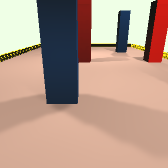
\includegraphics{Bilder/agent_input_image2.png}}\qquad
     \subfigure[Downsampled image]{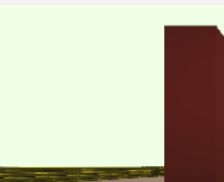
\includegraphics{Bilder/downsampled.png}}\\
     \subfigure[greyscale]{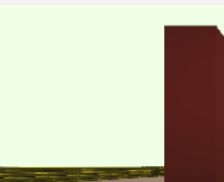
\includegraphics{Bilder/greyscaled.png}}\qquad
     \subfigure[histogram equalized image]{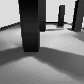
\includegraphics{Bilder/equalized.png}}
     \caption{4 Stages of preprocessing images for the CNN}
     \label{fig:4bildchen}
\end{figure}


\section{Training Process}


\subsection*{Training Parcours}
The PPO Reinforcement Learning algorithm requires the agent to be placed in a simulation environment similar to the evaluation environment to achieve good results. The agent will be placed in an arena with goal objects during training. In previous work \autocite{maximilian} two different training regimes were used, Single-Goal-Training and Full-Map-Training. In Single-Goal-Training the training was stopped after completing the first goal or upon collision. In Full-Map-Training the training was stopped after completing the whole map or upon collision. The reasoning behind Single-Goal-Training is that the agent will encounter a bigger variety of states during training since it will start at different positions in the map. However the Full-Map-Training scenario is closer to the evaluation scenario since the agent has to complete multiple goals in succession during evaluation.
Single-Goal-Training performed worse than Full-Map-Training in the previous work \autocite{maximilian} for all evaluation parcours except for the difficult one.

A third possible regime would be Full-Map-Training with randomized starting positions, this combines both approaches. The Single-Goal-Training is not strictly worse or better than Full-Map-Training. Therefore is not clear what training regime to chose for this thesis, therefore SGT, FMT and FMT with randomized starting positions will be compared during the experimentation phase.
% randomized starting positions also means start at random goals

\subsection*{Training Light Settings}
Since the agent utilizes a Convolutional Neural Network to be resilient towards changing light conditions it is also necessary to train the agent with varying light conditions, otherwise the adaptability of the CNN would not be fully utilized. This way the agent will be able to learn to generalize to different light conditions. The light conditions will be randomized for each training parcour.
Training with fixed light settings could also provide interesting insights when comparing the results to the results of training with varying light settings. If there is enough time the agent will be trained with fixed light settings as well. The comparison would show if the varying light settings during training helps for the generalization to different light settings.

% TODO put a figure with randomized light settings here
% maybe camera image from agents with different light settings

\begin{figure}
     \centering
     \subfigure[standard lighting]{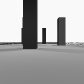
\includegraphics{Bilder/light_setting_standard.png}}\\
     \subfigure[reduced lighting]{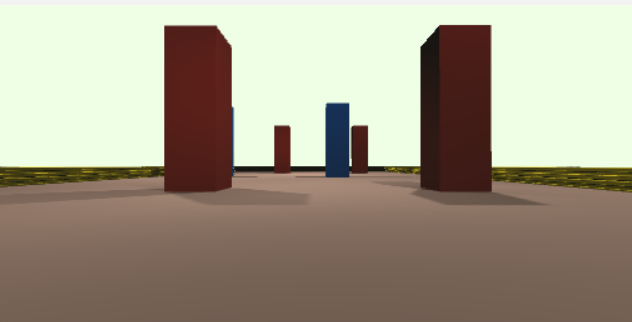
\includegraphics{Bilder/light_setting_reduced_lighting.png}}
     \subfigure[Increased lighting]{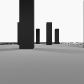
\includegraphics{Bilder/light_setting_increased_lighting.png}}
     \caption{different lightings TODO fix the images}
     \label{fig:3tracks}
\end{figure}

% TODO do we need an image equalization if the network is trained on varying light conditions?

\subsection*{Data Augmentation}
Convolutional Neural Networks require a lot of data to learn and generalize. Data augmentation is a technique to increase the amount of data available during training by applying transformations to the collected data. Collected data can be used to produce many more training examples by applying transformations such as rotation, translation, scaling, flipping and colour changes. In addition to providing a more diverse set of training data, this saves a lot of time since the new data points are not collected in simulation. \autocite{conditional_imitation_learning} employed a diverse set of data augmentation for their imitation learning approach that used a CNN.
During the training process the collected images will be augmented by applying random transformations to them. The transformations change the image similarly to how different environment conditions (e.g. lighting, camera quality and fog) might change the image. It is not yet decided which transformations will be used, possible candidates are changes in contrast, brightness and tone, as well as filters like Gaussian blur, Gaussian noise, salt-and-pepper noise.
Geometric transformations such as translations and rotations are not used since our control commands are not invariant to these transformations.


\begin{figure}
     \centering
     \subfigure[Original image]{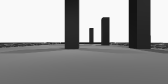
\includegraphics{Bilder/data_entry_original.png}}\\
     \subfigure[Gaussian Noise Mean 0 Sigma 5]{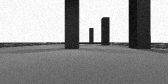
\includegraphics{Bilder/data_entry_augmented_gaussian_sigma_5.png}}\\
     \subfigure[salt-and-pepper noise]{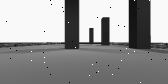
\includegraphics{Bilder/data_entry_augmented_salt_and_pepper.png}}
     \caption{Data augmentation examples}
     \label{fig:3tracks}
\end{figure}

% TODO find another paper with data augmentaton


\chapter{Experiment Description}
\label{cha:Experiments}

\section{Evaluation metrics}

\subsection{success\_rate}
The primary metric of evaluation for the developed agents is the $success\_rate$. The $success\_rate$ is defined as the ratio of successful episodes to the total number of episodes. An episode is considered successful if the agent passes through all three goals within the time limit \ref{time_limit}. Collisions of the agent do not disqualify an episode from being succesful, as long as the agent passes all goals.

\subsection{goal\_completion\_rate}

The $goal\_completion\_rate$ is defined as the ratio of passed goals to the total number of goals in the episodes. The $goal\_completion\_rate$ is a more fine-grained metric than the $success\_rate$. However the two metrics are closely related as a high $success\_rate$ implies a high goal\_completion\_rate. The major advantage of the $goal\_completion\_rate$ is that it can used to measure the progress of an agent during training more accurately.
The $goal\_completion\_rate$ would increase when the agent is able to pass more goals on average, whereas the $success\_rate$ would only increase when the agent is able to pass all goals in an episode more often. The $goal\_completion\_rate$ captures learning progress earlier in training. This behaviour can be observed in training runs, shown in \ref{fig:success_rate_vs_goal_completion_rate}.


\begin{figure}
    \centering
    \subfigure[success\_rate]{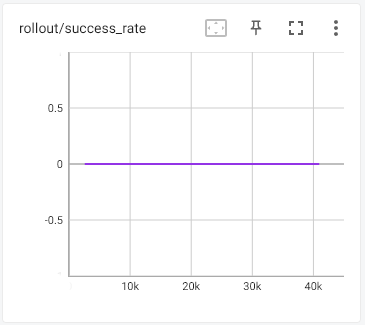
\includegraphics[width=0.3\textwidth]{Bilder/metrics/sr_vs_gcr_success_rate.PNG}}
    \subfigure[goal\_completion\_rate]{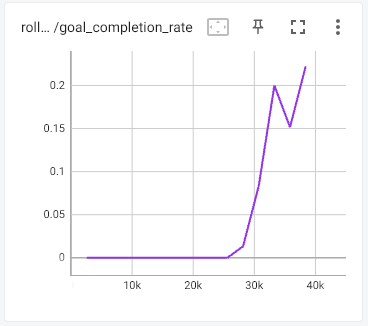
\includegraphics[width=0.3\textwidth]{Bilder/metrics/sr_vs_gcr_goal_completion_rate.PNG}}
    \caption{Difference in success rate and goal completion rate during early stages of training.}
    \label{fig:success_rate_vs_goal_completion_rate}
\end{figure}
% diese Bilder funktionieren nur für frühe Episoden, später sind die Werte sehr gleich

\subsection{collision\_rate}

The $collision\_rate$ is defined as the ratio of episodes with one or more collisions to the total number of episodes. The $collision\_rate$ is a measure of the agent's ability to avoid obstacles. The $collision\_rate$ is a secondary metric. The $collision\_rate$ is used in combination with the $success\_rate$ to determine the agent's performance.
The collision rate is also very useful during the training of the agent. If the agent's goal completion rate is low and there are no collisions, the agent might be stuck in a local optimum. In one such situation, the agent turned on the spot avoiding any collisions and did not move forward at all.
The collision rate can be used to detect such situations, the training process can then be adjusted accordingly.


\section{Basic evaluation algorithm}
\label{sec:basic_evaluation_algorithm}

This section explains the most important component of the evaluation algorithms. It explains how the policy's performance is evaluated on a specific light and difficulty setting. The sampling mode, jetbot name and other policy parameters can also be specified \ref{table:basic_eval_algorithm_parameters}. This basic component is widely used in the following tests.


\begin{table}
    \begin{center}
        \begin{tabular}{|| c | p{0.20\linewidth} | p{0.4\linewidth} ||}
            \hline
            Parameter name                     & Options              & Explanation                                                                                  \\ [0.5ex]
            \hline\hline
            \multirow{1}{*}{n\_eval\_episodes} & any positive integer & Amount of episodes to use for evaluation                                                     \\
            \hline
            \multirow{3}{*}{difficulty}        & easy                 & \multirow{3}{\linewidth}{Determines tracks used for episodes}                                \\\cline{2-2}
                                               & medium               &                                                                                              \\\cline{2-2}
                                               & hard                 &                                                                                              \\
            \hline
            \multirow{3}{*}{light\_setting}    & bright               & \multirow{3}{\linewidth}{Determines light setting for episodes}                              \\\cline{2-2}
                                               & standard             &                                                                                              \\\cline{2-2}
                                               & dark                 &                                                                                              \\
            \hline
            \multirow{2}{*}{jetbot\_name}      & DifferentialJetBot   & \multirow{2}{\linewidth}{JetBot version for episodes}                                        \\\cline{2-2}
                                               & FourWheelJetBot      &                                                                                              \\
            \hline
            \multirow{2}{*}{deterministic}     & True                 & \multirow{2}{\linewidth}{If True, use deterministic sampling for policy actions}             \\\cline{2-2}
                                               & False                &                                                                                              \\
            \hline
            \multirow{2}{*}{use\_fresh\_obs}   & True                 & \multirow{2}{\linewidth}{If True, request new fresh observation from Unity before inference} \\\cline{2-2}
                                               & False                &                                                                                              \\
            \hline
            \multirow{2}{*}{record\_videos}    & True                 & \multirow{2}{\linewidth}{If True, record videos}                                             \\\cline{2-2}
                                               & False                &                                                                                              \\
            \hline
            \multirow{2}{*}{log}               & True                 & \multirow{2}{\linewidth}{If True, log all metrics to tensorboard}                            \\\cline{2-2}
                                               & False                &                                                                                              \\
            \hline
            \multirow{1}{*}{step}              & any positive integer & step for Tensorboard logging                                                                 \\
            \hline
        \end{tabular}
    \end{center}
    \caption{Basic evaluation algorithm parameters}
    \label{table:basic_eval_algorithm_parameters}
\end{table}



The agent is evaluated by running a fixed number of episodes for the specific light and difficulty settings. The amount of episodes that the agent is evaluated on is defined by the config parameter $n\_eval\_episodes$. As described in \ref{cha:env_description}, each difficulty setting includes a number of unique tracks. Furthermore the initial starting rotation is parameterized by the config parameter $spawn\_point$.

The tracks and starting positions for the agent are generated by the algorithm shown in \ref{fig:generate_track_rotation}. The algorithm divides the random interval specified by the spawn point parameter into $n\_eval\_episodes$ equal parts. These spawn rotations are then each assigned a track in repeating order.
This algorithm ensures that the agent is evaluated on the full range of unique tracks and spawn points.
It also makes the evaluations comparable, as the same combinations of tracks and spawn points are used for each agent evaluation.

The evaluation algorithm initializes $n\_eval\_episodes$ environments with the specified light settings. The obstacles and agents are then placed in the environments according to the generated map and rotation pairs. The evaluation episodes are started and the agents act in their environment until their episodes are terminated. The agent's actions are sampled deterministically or non-deterministically depending on the function call's parameter. The agent is executed in fresh or non-fresh observation mode depending on the function call's parameter.

The $success\_rate$ and $collision\_rate$ are calculated from the executed episodes, both metrics are returned to the caller. Many other metrics such as the $goal\_completion\_rate$ and $average\_episode\_length$ are calculated, they are logged to tensorboard if $log==True$.


\section{Question 1 - Model evaluation track difficulties}

The agent is evaluated on all three different difficulty settings to determine if the agent is successful in completing the tracks.
The Basic evaluation algorithm is used with the standard light setting for each of the three difficulty settings.
The policy is executed in non deterministic mode. This mode showed slight improvements over deterministic sampling, see \ref{sec:deterministic_check}



\paragraph{Test parameters}

100 episodes are evaluated for every difficulty setting. The $spawnOrientation$ from the training process is reused for the evaluation.


\section{Question 2 - Model evaluation all light settings}

The agent is evaluated on every combination of light and difficulty settings. The Basic evaluation algorithm is used for these evaluations.
The $success\_rate$ metric is collected for each combination of light and difficulty settings separately. The collected $success\_rates$ are then averaged to produce aggregate $success\_rates$ for each light setting and difficulty setting as well as the $total\_success\_rate$. All collected and aggregate $success\_rates$ are shown in \ref{table:success_rates_system}.
The experiment shwos if the agent is able to adapt to different light settings and if the agent's performance is influenced by the light settings.

\begin{table}
    \begin{center}
        \resizebox{\textwidth}{!}{%
            \begin{tabular}{|| c | c | c | c | c ||}
                \hline
                \makecell{}       & bright                  & standard                  & hard                  & \makecell{aggregate \\ success\_rates} \\ [0.5ex]
                \hline\hline
                \makecell{easy}   & success\_easy\_bright   & success\_easy\_standard   & success\_easy\_dark   & success\_easy       \\
                \hline
                \makecell{medium} & success\_medium\_bright & success\_medium\_standard & success\_medium\_dark & success\_medium     \\
                \hline
                \makecell{hard}   & success\_hard\_bright   & success\_hard\_standard   & success\_hard\_dark   & success\_hard       \\
                \hline
                \makecell{aggregate                                                                                                   \\ success\_rates}  & success\_bright & success\_standard & success\_dark & total\_success\_rate \\
                \hline
            \end{tabular}}
    \end{center}
    \caption{Collected and aggregate success\_rate metrics}
    \label{table:success_rates_system}
\end{table}


\section{Question 3 - Investigating the feasibility of transfering the policy to a physical robot.}

Previous sections describe how a policy was developed that can be used to control an agent in a simulated environment. This section describes how I will investigate the feasibility of transfering the developed policy onto physical devices. The simulated agent was modeled after a Nvidia JetBot. The Nvidia JetBot is a small robot that is equipped with a camera, a processing unit and two motors that can be controlled independently.
The Nvidia Jetbot is designed to be able to execute AI software. However the limited computational power of the JetBot raises the question whether the developed policy can be transfered to the JetBot.

The developed policy takes a camera image from the front of the agent as input and applies preprocessing steps to the image. The preprocessed image is then processed by a convolutional neural network that outputs two acceleration values, one for each motor. The acceleration values are applied to the motors for a fixed amount of time. While the agent is moving, the camera image is constantly updated and the policy is applied to the new image. It is crucial that the agent's policy can be computed quick enough to be able act in real time.

\subsection*{Effects of insufficiently slow policy computation}
If the jetbot is not able to compute the developed policy in the required time, there are two options that do not require changes to the developed/trained policy. The first option is to stop the motors until the policy is computed and then apply the acceleration values. This would make the jetbot movement overall slower and less smooth.
The second option is to apply the last computed acceleration values to the motors until the new policy is computed. This could result in a degradation of the jetbot's performance since the actions would be less accurate.
The two options are shown with visual representations in \ref{fig:slow_policy_computation}.


% gif splitter
% https://ezgif.com/split


\newcommand{\spc}[2]{\subfigure[#1]{\includegraphics[width=0.2\textwidth]{Bilder/slow_policy_computation/#2.png}}}
%\newcommand{\spc}[2]{\begin{subfigure}{.5\textwidth}\centering\includegraphics[width=0.2\textwidth]{Bilder/slow_policy_computation/#2.png}\caption*{#1}\end{subfigure}}
% trying to remove a), b) ... https://tex.stackexchange.com/questions/165508/remove-a-b-from-subfigure-numbering-but-keep-the-subfigure-caption

\begin{figure}

    \begin{center}
        \begin{tabular}{|| c | c | c ||}
            \hline
            Policy computation in time                                  & \makecell{Option 1:                                                                                                   \\ Wait} & \makecell{Option 2:\\ Apply previous outputs}  \\ [0.5ex]
            \hline\hline
            \spc{Start}{start}                                          & \spc{Start}{start}                                          & \spc{Start}{start}                                      \\
            \hline
            \spc{Agent turns right}{agent_turns_right}                  & \spc{Agent turns right}{agent_turns_right}                  & \spc{Agent turns right}{agent_turns_right}              \\
            \hline
            \spc{Agent stops turning and goes strait}{agent_turns_left} & \spc{Agent waits}{agent_turns_right}                        & \spc{Agent continues to turn}{agent_fails_to_turn_left} \\
            \hline
            \spc{Agent continues}{agent_continues_properly}             & \spc{Agent stops turning and goes strait}{agent_turns_left} & \spc{Agent crashes}{agent_crashes}                      \\
            \hline
            \makecell{Agent moves properly.}                            & \makecell{Agent overall speed is reduced.}                  & \makecell{Agent behaviour is changed.}                  \\
            \hline
        \end{tabular}
    \end{center}
    \caption{Possible effects of slow policy computation on the performance.}
    \label{fig:slow_policy_computation}
\end{figure}



\subsection{Policy Replay Experiment}
\label{sec:experiments_policy_replay}

This experiment examines the processing capabilities of the Nvidia Jetbot in the context of policy computation. The goal of this experiment is to determine if the policy can be computed on the jetbot hardware in real time. This would allow for a transfer of the developed policy to the physical agent without resorting to the two options highlighted in the previous section.

The experiment is conducted by recording the agent's actions in simulation and replaying them on the Nvidia Jetbot. The experiment measures the time it takes to replay the recorded actions on the jetbot.

\paragraph{Recording Episodes}

Episodes are recorded in the simulation environment. The policy that is used for the recording is saved for later replay on the jetbot.
The recordings consist of the agent's camera images and the corresponding policy outputs. The camera images are saved without the proprocessing steps applied. These images represent the raw camera input that the jetbot agent would recieve in real time. The policy outputs are saved to verify the accuracy of the policy on the jetbot.

The episode recordings and policy are then transfered to the jetbot and executed.

\paragraph{Replaying Episodes}

The recorded episodes are replayed on the jetbot. The policy from the recording is used to execute the replays on the jetbot. All recorded images and policy outputs are loaded into memory in preparation of an episode replay.
The episodes are replayed step by step. The replay of a step consists of all the processing to obtain new acceleration values from a camera image. Image preprocessing and memory mechanism are executed for each step according to the specifications of the saved policy. The policy outputs are then computed. The computed policy outputs and the recorded policy outputs are used to verify the accuracy of the saved policy on the jetbot.

The transfer of a neural network to a new device can result in different outputs due to different hardware. The computed and saved policy outputs are compared to determine the accuracy of the policy on the jetbot.

The test measures the time it takes to replay the recorded steps on the jetbot.
The measured times are compared against the $fixedTimestepsLength$ parameter of the recorded policy.


\paragraph{Test Dataset}

Episodes of all difficulty and light setting combinations are recorded to have a diverse set of data to evaluate. The episodes are recorded with the same policy as question 1 and 2, the most successful policy.

% we always record in the use_fresh_obs mode


\section{Other Experiments}

\subsection{Sampling mode performance test}
\label{sec:deterministic_check}

The PPO policy produces an action distribution when given an input observation. The action distribution is sampled to obtain an action for the agent to execute in the environment. The distribution can be sampled deterministically or non-deterministically. Deterministic sampling returns the most likely action, indicated by the mean of the distribution. Non-deterministic sampling returns a sample from the distribution according to the distribution's probabilities. This results in different output actions for the same observations. The PPO policy uses non-deterministic sampling during training to explore the action space.

While the exploration caused by non-deterministic sampling is beneficial during training, it could be detrimental during evaluation. This exploration could lead the agent to take actions that are not optimal for the given observation and result in a lower $success\_rate$. Non-deterministic sampling can also be used during evaluation to reduce overfitting. This has been used in the Atari paper \textcite{atari} and the human-level control paper \textcite{human_level_control}. The environments examined in these papers are deterministic with identical starting states. Therefore a deterministic policy would result in identical results for the individual evaluation episodes.

Due to the difference in environment properties between the JetBot environment and the Atari environment, it is not clear if deterministic or non-deterministic sampling is better for the JetBot environment. The sampling mode performance test evaluates the agent with deterministic and non-deterministic sampling to determine if the agent's performance is affected by the sampling method.

The sampling mode performance test uses the Basic evaluation algorithm to evaluate an agent with derministic and non-deterministic sampling for each difficulty level. The test evaluates the agents only using the standard light setting to save evaluation time. The success rates for the two sampling modes are compared to determine if the agent's performance is influenced by the sampling method.



% atari.pdf and human_level_control.pdf uses epsilon greedy during evals (their environment is deterministic, thus using a deterministic policy would result in the same results for every episode)

% default we use non deterministic, as that has shown (slightly) better results and is also used by atari paper


\subsection{Identical start condition Test}

The environment is simulated in Untiy. The unity game engine is not fully deterministic \autocite{unity_fixed-update}. This means identical actions in identical environment states can result in slightly different environment states. In addition the policy evaluation may use non-deterministic sampling for selecting actions \ref{sec:action_sampling}. This results in different actions for identical observations. 

Therefore, episodes with identical starting conditions could result in different outcomes. This would be problematic when evaluating the agent since the evaluation results would not be reliable.

The identical start condition test evaluates the agent on multiple episodes with identical starting conditions. The episode results are analysed to see if the policy is consistent when given identical starting conditions. If the policy is inconsistent given identical starting conditions, the evaluation results according to \ref{sec:basic_evaluation_algorithm} are not reliable. The evaluation algorithm described in \ref{sec:basic_evaluation_algorithm} evaluates the agent on a series of different starting conditions, each starting condition is unique and only evaluated once.

This test runs multiple episodes with identical start conditions and analyses the episodes. The episode results are characterized and grouped. The groups are then analysed to determine if the agent's performance is consistent given identical starting conditions. Ideally all episodes would result in the same outcome.
The episode results are characterized by the endEvent, collision and the three goals' completion.


\subsection{Fresh Observation Test}

In the standard reinforcement learning algorithms each step transition results in a new observation that represents the environment's new state. Calls to the Unity environment and the step transitions in the environment take time. In order to speed up the training process the step calls to the simulated environment have been implemented in a non-blocking way. This means the step calls return before the entire step transition has been completed. The observation after the step transition is not yet available when the call returns. The observation returned by the step call is the observation of the environment at the beginning of the step transition. This observation does not capture the changes that have occurred in the environment during the step transition. The full changes are then visible to the agent after the next step has completed.

The option $use\_fresh\_obs$ controls what observations the policy uses to produce the next actions. If $use\_fresh\_obs$ is set to false, the observation returned by the last step call is used. If $use\_fresh\_obs$ is set to true, a new observation is requested from the Unity simulation.

The fresh observation test evaluates a trained policy with both $use\_fresh\_obs$ settings to determine if the agent's performance is influenced by the freshness of the observations. The trained policy used one setting of the $use\_fresh\_obs$ parameter during training. The test shows if there is a difference in the agent's performance when using the other setting. The test evaluates the agent on light and difficulty settings following the evaluation algorithm described in \ref{sec:basic_evaluation_algorithm}.


\subsection{JetBot generalization Test}

There are two versions of the agent in simulation, the DifferentialJetBot and FourWheelJetBot \ref{fig:jetbots}. The DifferentialJetBot has two front wheels that are accelerated independently for steering. The FourWheelJetBot angles its two front wheels for steering. These differences can result in different agent movement for the same acceleration inputs. The DifferentialJetBot is used during training as this is closer to the physical jetbot availible at the Scads.AI.
The agent's movement behaviour influences the developed policy. The agent learns from the changes in the environment that result from its actions. The policy might perform worse when the agent's movement behaviour changes.

A policy trained on the DifferentialJetBot might not generalize well to the FourWheelJetBot and vice versa. The JetBot generalization test evaluates the trained policy on both JetBot versions to determine if the policy can be transfered to the FourWheelJetBot without retraining. The test evaluates the agent on the different difficulty levels using the basic evaluation algorithm described in \ref{sec:basic_evaluation_algorithm}. The test is only executed for the standard light condition to save time.





%\chapter{Methods}
%\label{cha:Methods}
%\lipsum \autocite{DBLP:books/sp/HarderR01}

\section{Investigating the feasibility of transfering the policy to a physical robot.}

Previous sections describe how a policy was developed that can be used to control an agent in a simulated environment. This section describes how I will investigate the feasibility of transfering the developed policy onto physical devices. The simulated agent was modeled after a Nvidia JetBot. The Nvidia JetBot is a small robot that is equipped with a camera, a processing unit and two motors that can be controlled independently. 
The Nvidia Jetbot is designed to be able to execute AI software. However the limited computational power of the JetBot raises the question whether the developed policy can be transfered to the JetBot. 

The developed policy takes a camera image from the front of the agent as input and applies preprocessing steps to the image. The preprocessed image is then processed by a convolutional neural network that outputs two acceleration values, one for each motor. The acceleration values are applied to the motors for a fixed amount of time. While the agent is moving, the camera image is constantly updated and the policy is applied to the new image. It is crucial that the agent's policy can be computed quick enough to be able act in real time. 

\subsection{effects of insufficiently slow policy computation}
If the jetbot is not able to compute the developed policy in the required time, there are two options that do not require changes to the developed/trained policy. The first option is to stop the motors until the policy is computed and then apply the acceleration values. This would make the jetbot movement overall slower and less smooth.
The second option is to apply the last computed acceleration values to the motors until the new policy is computed. This could result in a degradation of the jetbot's performance since the actions would be less accurate.
The two options are shown with visual representations in \ref{fig:slow_policy_computation}.


% gif splitter
% https://ezgif.com/split



\newcommand{\spc}[2]{\subfigure[#1]{\includegraphics[width=0.2\textwidth]{Bilder/slow_policy_computation/#2.png}}}
%\newcommand{\spc}[2]{\begin{subfigure}{.5\textwidth}\centering\includegraphics[width=0.2\textwidth]{Bilder/slow_policy_computation/#2.png}\caption*{#1}\end{subfigure}}
% trying to remove a), b) ... https://tex.stackexchange.com/questions/165508/remove-a-b-from-subfigure-numbering-but-keep-the-subfigure-caption

\begin{figure}
    
    \begin{center}
    \begin{tabular}{|| c | c | c ||} 
        \hline
        Policy computation in time & \makecell{Option 1: \\ Wait} & \makecell{Option 2:\\ Apply previous outputs}  \\ [0.5ex] 
        \hline\hline
        \spc{Start}{start} &  \spc{Start}{start} & \spc{Start}{start} \\ 
        \hline
        \spc{Agent turns right}{agent_turns_right} & \spc{Agent turns right}{agent_turns_right} & \spc{Agent turns right}{agent_turns_right} \\
        \hline
        \spc{Agent stops turning and goes strait}{agent_turns_left} & \spc{Agent waits}{agent_turns_right} & \spc{Agent continues to turn}{agent_fails_to_turn_left} \\
        \hline
        \spc{Agent continues}{agent_continues_properly}  & \spc{Agent stops turning and goes strait}{agent_turns_left} & \spc{Agent crashes}{agent_crashes} \\
        \hline
        \makecell{Agent moves properly.}  & \makecell{Agent overall speed is reduced.} & \makecell{Agent behaviour is changed.} \\
        \hline
    \end{tabular}
    \end{center}
    \caption{Effects of slow policy computation on the performance.}
    \label{fig:slow_policy_computation}
\end{figure}






\include{Inhalt/EvaluationAndExperimentation}

\chapter{Results}
\label{cha:Results}

This chapter presents the results of the experiments conducted in this project. The first three experiments were designed to answer the research questions posed in chapter \ref{cha:ResearchGoals} specifically. 

The experiments were conducted using the policy that was developed as a result of the parameter experimentation \ref{sec:most_successful_policy}. This policy was trained exclusively on hard tracks with all light settings. The histogram equalization preprocessing step was used during training.


\section{Eval for question 1 - \questionOne}

The trained policy was evaluated on tracks of all difficulty settings with the standard light setting using the Basic Evaluation algorithm \ref{sec:basic_evaluation_algorithm} with 100 episodes per setting. The success rates for the different difficulty settings are shown in figure \ref{fig:result_success_rates_standard}. Example videos of the agent's behaviour during evaluation can be found in the appendix \ref{cha:example_videos}.

\subsection{Experiment Results}

\begin{figure}
    \centering
    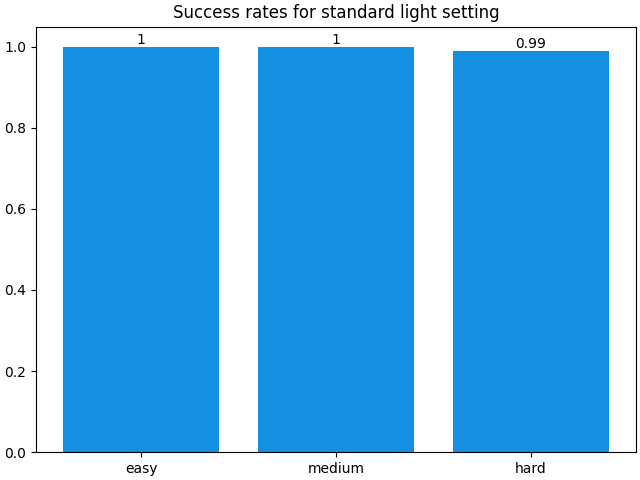
\includegraphics[width=0.45\textwidth]{Bilder/notebook_images/hardDistanceMixedLight_eval_standard_success_rates_barplot.png}
    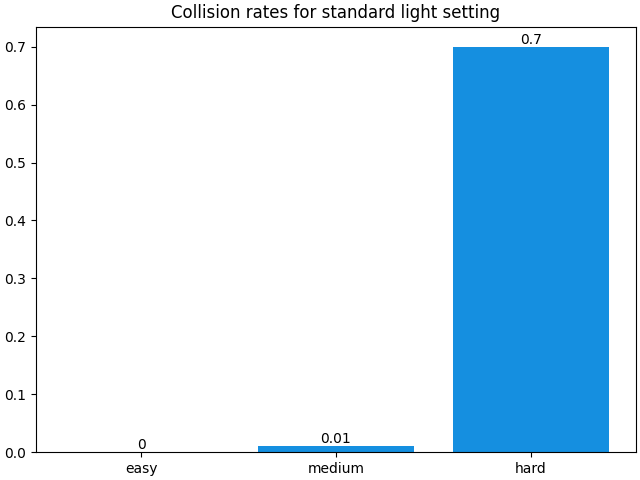
\includegraphics[width=0.45\textwidth]{Bilder/notebook_images/hardDistanceMixedLight_eval_standard_collision_rates_barplot.png}
    \caption{Success and collision rates for standard light setting.}
    \label{fig:result_success_rates_standard}
\end{figure}


The policy completed the easy, medium and hard tracks with a succes\_rate of 100\%, 100\% and 99\%. 
The collision\_rates were 0\%, 1\% and  70\%. Especially for the hard difficulty setting, the agent does not avoid collisions completely. 

The analysis of successful episodes with collisions shows that these collisions are only minor collisions. The agent passes the goals very close to the goal post that is closer to the arena middle \ref{fig:agent_behaviour}. This often results in collisions with the goal obstacles at its side.

\begin{figure}
    \centering
    \subfigure[Agent passes the goal close to the arena middle]{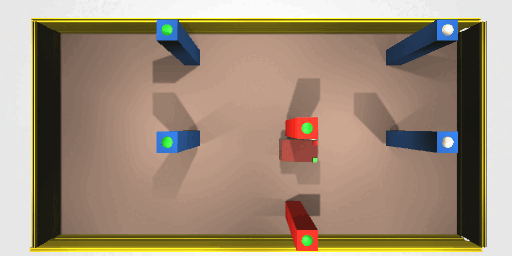
\includegraphics[width=0.45\textwidth]{Bilder/example_goal_passing_close_to_middle.png}}
    \subfigure[Agent may collide with goal post at the side]{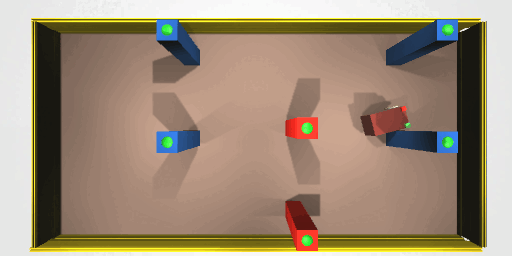
\includegraphics[width=0.45\textwidth]{Bilder/example_minor_collision_topview_frame_1295.png}}
    \caption{Goal passing behaviour of the trained agent}
    \label{fig:agent_behaviour}
\end{figure}

The unsuccessful episodes of hard tracks were analysed to determine why the agent does not reach 100\% success rates. The analysis showed that the agent has frontal collisions with the first goal post at the agents side \ref{fig:unsuccessful_episodes}. This occurs only when the agent is spawned with an extreme rotation. The agent cannot complete the tracks in about 40\% of episodes with the maximum rotation of $15^{\circ}$.

\begin{figure}
    \centering
    \subfigure[Agent is spawned with extreme rotation]{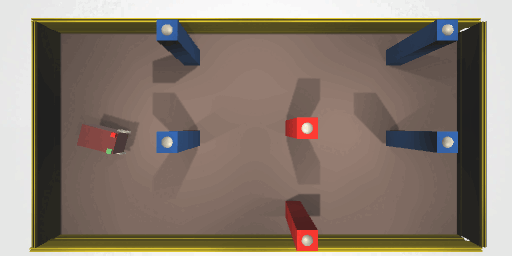
\includegraphics[width=0.3\textwidth]{Bilder/extremeSpawnRot_agent_initial.png}}
    \subfigure[Agent approaches first goal post]{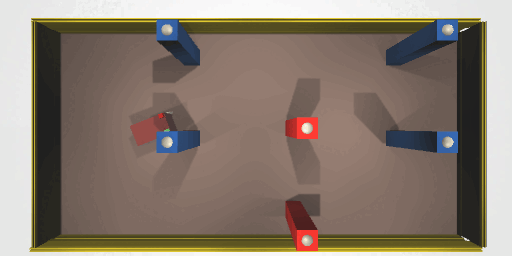
\includegraphics[width=0.3\textwidth]{Bilder/extremeSpawnRot_agent_turns.png}}
    \subfigure[Agent collides with first goal post and remains stuck]{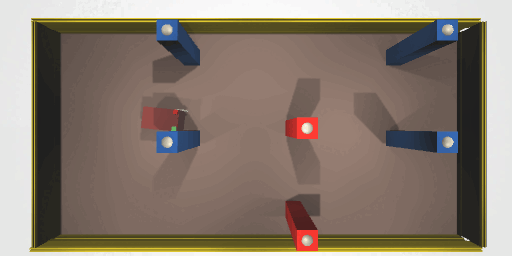
\includegraphics[width=0.3\textwidth]{Bilder/extremeSpawnRot_agent_collides.png}}
    \caption{Analysis of unsuccessful episodes}
    \label{fig:unsuccessful_episodes}
\end{figure}



\subsection{Conclusion}

The trained policy is able to complete all difficulty levels very reliably. The policy reached success rates of 100\%, 100\% and 99\% for easy, medium and hard tracks. The end-to-end trained \ac{CNN} policy proves to be very effective at solving the autonomous driving task.

The policy outperforms previous work at the ScaDS.AI by \textcite{maximilian}. The policies developed by \textcite{maximilian} reached success rates of 99\%, 89\% and 64\% for easy, medium and hard tracks.

The policy was trained on the difficult setting only. The policy did not see easy and medium difficulty tracks before the evaluation. The policy is able to generalize to tracks of lower difficulty.

\section{Eval for Question 2 - \questionTwo}

The most succesfull model was used to evaluate the agent's performance under different light settings. The agent was evaluated on the standard, dark and bright light settings. Each combination of difficulty and light setting was evaluated with the Basic Evaluation Algorithm for 100 episodes. The success rates for the different light settings are shown in figure \ref{fig:result_success_rates_lightSettings}.


\subsection{Experiment Results}

\begin{figure}
    \centering
    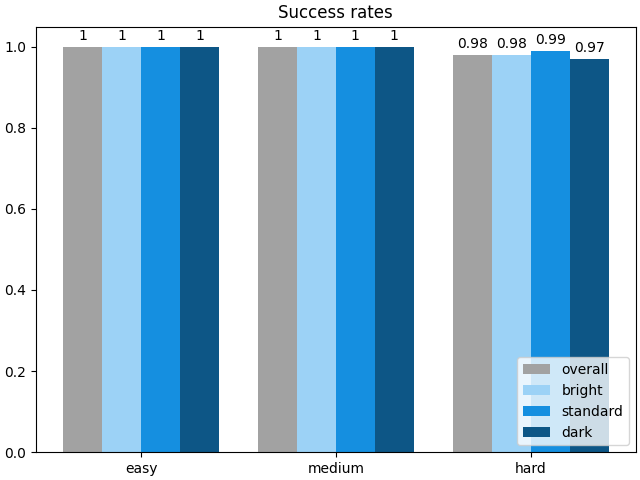
\includegraphics[width=0.45\textwidth]{Bilder/notebook_images/hardDistanceMixedLight_eval_all_success_rates_barplot.png}
    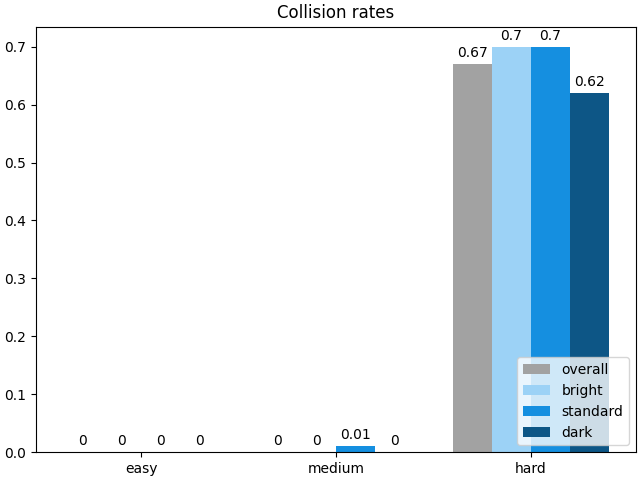
\includegraphics[width=0.45\textwidth]{Bilder/notebook_images/hardDistanceMixedLight_eval_all_collision_rates_barplot.png}
    \caption{Success and collision rate comparisons for light settings.}
    \label{fig:result_success_rates_lightSettings}
\end{figure}

The success rates for all light and difficulty settings are very high at above 95\%. The agent completed the easy and medium tracks with a success rate of 100\%. The light setting had no influence on the success\_rate for the easy and medium tracks.
The evaluations for the bright and dark light settings show slight decreases in performance compared to the standard light setting for hard tracks. The success\_rate of hard tracks in the bright and dark light setting was 98\% and 97\%.

The collision rates are very low for the easy and medium tracks. All tracks in these settings were solved without collisions except for the medium tracks with the standard light setting. This medium standard evaluation had a collision rate of 1\%.
The collision rates for the hard tracks are quite high at 70\% for the standard light setting. The bright and dark light settings are very high as well with 70\% and 62\%.

Across all light and difficulty settings the overall success rate is almost 100\% and the overall collision rate is 22\%.

\subsection{Conclusion}

The policy was able to complete the tracks very reliably under the different light settings. The light setting only had a minor impact on the success rate.
Furthermore the different light settings did not lead to an overall increase in collisions.

The developed policy was trained following the experiments in the previous chapter. The agent used the histogram equalization preprocessing step and mixed light settings during training. Using these settings the policy was able to learn to navigate the tracks with all light conditions.


\section{Eval for Question 3 - \questionThree}

The most successful model was used to record replays of the agent's behaviour. This most successful model used a $fixedTimestepLength$ of $0.3$ seconds. This means the hardware has to able to make a decision every $0.3$ seconds to be considered fast enough.

Five episodes were recorded for each difficulty and light setting combination. As expected from the previous evaluations of the policy, the replay episodes had a very high success\_rate of 100\%. The recorded episodes were then replayed on the Nvidia Jetbot. The time it took to replay the episodes was measured \ref{fig:result_replay_times}. The policy outputs from the replay were compared to the policy outputs from the recordings \ref{fig:result_replay_outputs}. The differences are caused by the hardware and software differences between the training and the replay environment.


\begin{figure}
    \centering
    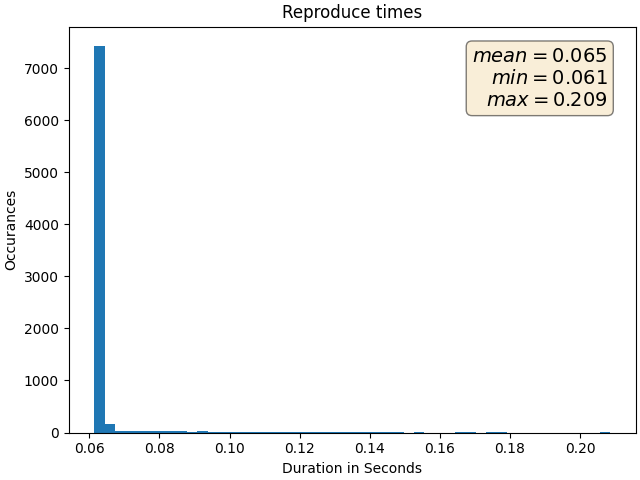
\includegraphics[width=0.5\textwidth]{Bilder/notebook_images/replay_times.png}
    \caption{Replay times on jetbot hardware}
    \label{fig:result_replay_times}
\end{figure} % a chart showing the replay times (max, min, mean)


\begin{figure}
    \centering
    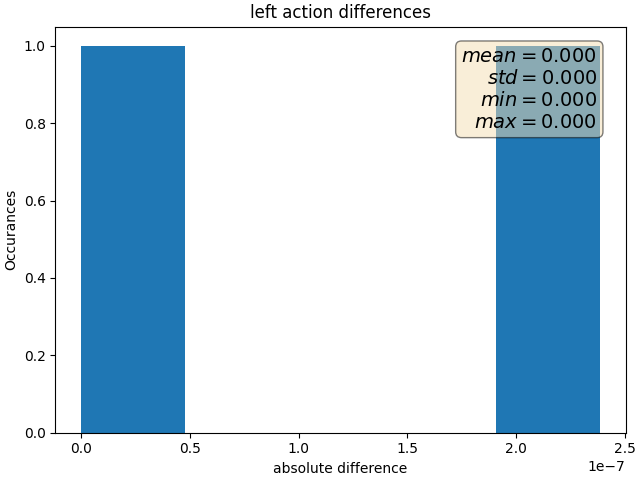
\includegraphics[width=0.45\textwidth]{Bilder/notebook_images/replay_outputs_action_left.png}
    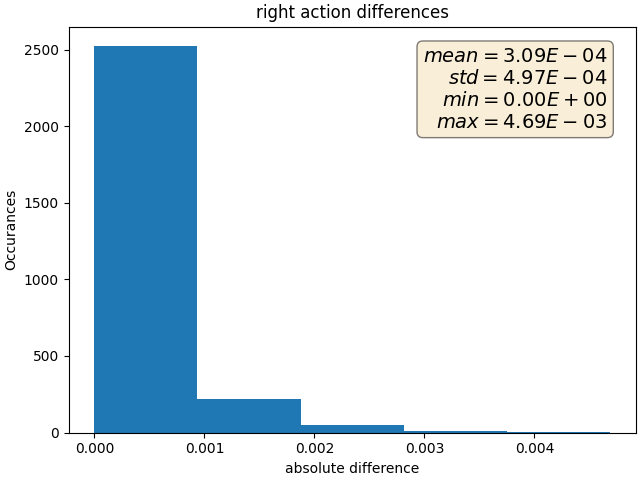
\includegraphics[width=0.45\textwidth]{Bilder/notebook_images/replay_outputs_action_right.png}
    \caption{Differences in policy outputs between recordings and replays on jetbot hardware}
    \label{fig:result_replay_outputs}
\end{figure} % a chart showing the replay outputs


\subsection{Experiment Results}

\paragraph{Replay times}

The replay times for the recordings on jetbot hardware are shown in figure \ref{fig:result_replay_times}. The maximum duration was $0.216$ seconds. The mean is much lower at $0.067$ seconds. The plot shows that the maximum duration was an extreme outlier.
Given the $fixedTimestepLength$ of $0.3$ seconds and the maximum duration of $0.216$ seconds, the hardware is fast enough to replay the episodes. This leaves at least $0.084$ seconds for the agent to receive an image from the camera and send the new instruction to the motors.

The cameras used in the nvida jetbot are capable of capturing images with a resolution of $1280x720$ pixels at $60$ frames per second. This means the camera can capture an image every $0.0166$ seconds. The hardware is quick enough to compute actions in real time.

% times replay hardDistanceMixedLight: min 0.06319522857666016, mean 0.06662133265668013, max 0.21592259407043457

\paragraph{Policy Outputs}

The policy outputs from the recordings and the replays on jetbot hardware are nearly identical. The differences are shown in figure \ref{fig:result_replay_outputs}. The outputs were reproduced very closely. The maximum difference was $4.69e-03$.  This is difference is negligeable compared to the range of policy outputs $[-1,1]$.

% left action differences min [0.], max [0.00433731], mean 0.00030147546203806996, std 0.0004885991802439094
% right action differences min [0.], max [0.00468674], mean 0.00030857478850521147, std 0.000496754830237478

\subsection{Discussion}

The jetbot hardware is capable enough to compute the policy in real time. The differences of the policy outputs between the recordings and the replays are very small, the policy outputs were reproduced very closely. This suggests the differences in hardware and software do not impact the policy significantly.

\section{Other Experiments}

\subsection{Sampling Mode Performance Test}
\label{ref:sampling_mode_test_results}

The sampling mode performance test uses the Basic evaluation algorithm to evaluate an agent with derministic and non-deterministic sampling for each difficulty level. The success rates for the two sampling modes are compared to determine if the agent's performance is influenced by the sampling method. The sampling mode test was executed for all agents during the experimentation phase of this project using standard light.

\paragraph{Results}
The tests showed that the difference in performance for the sampling modes was very small for the trained policies. The results showed empirically that non-deterministic sampling leads to better success rates. Nevertheless some policies performed slightly worse using the non-deterministic sampling mode. The success rate was on average 1.7\% higher when using non-deterministic sampling. The biggest difference was 2.6\% for the medium difficulty setting \ref{fig:deterministic_check_result}.

\begin{figure}
    \centering
    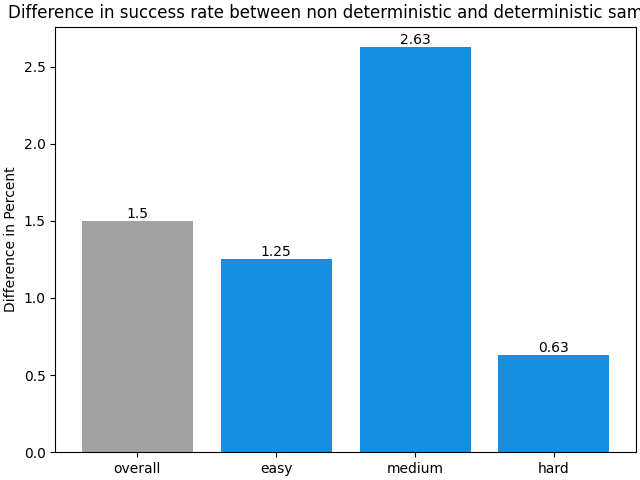
\includegraphics[width=0.8\textwidth]{Bilder/notebook_images/deterministic_check_results.png}
    \caption{Results of the deterministic check across all evaluations during the experimentation phase}
    \label{fig:deterministic_check_result}
\end{figure}

\paragraph{Discussion}
The test indicates that the non-deterministic sampling mode performes better, although the differences in performance are quite small. Given these results, the main evaluations for question 1 and 2 were conducted with non-deterministic sampling.

\subsection{Identical Start Condition Test}

The environment is not 100\% deterministic. This is due to the environment implementation in Unity \autocite{unity_fixed-update}. The environment uses physics simulations which are not fully deterministic. In addition the policy's actions are sampled non-deterministically during the evaluation.
This means that identical start conditions of an episode may result in different trajectories and results. This test evaluates the impact of the non-deterministic environment and sampling on the agent's behaviour. 

The agent with \ac{HX-P} is placed in the same start conditions for 100 episodes. The starting conditions entail the selected track, light condition and the agent's starting rotation. The test was executed for the hardBlueFirstRight trach with the standard lighting. Three starting rotations were used \ref{fig:identical_start_conditions_test_rotations}.
The episode results are compared.

\begin{figure}
    \centering
    \subfigure[-15°]{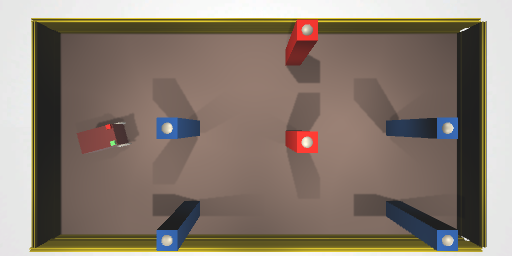
\includegraphics[width=0.3\textwidth]{Bilder/image_printer_images/identical_start_conditions/hardBlueFirstRight_minus15.png}}
    \subfigure[0°]{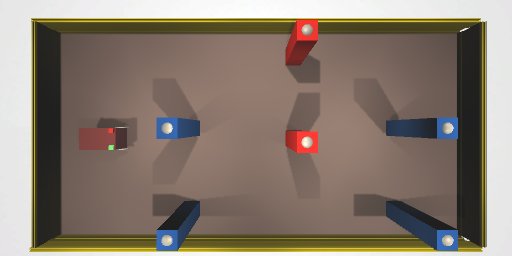
\includegraphics[width=0.3\textwidth]{Bilder/image_printer_images/identical_start_conditions/hardBlueFirstRight_0.png}}
    \subfigure[15°]{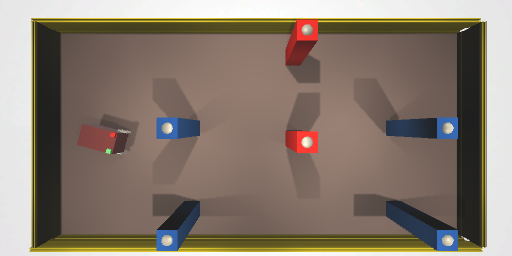
\includegraphics[width=0.3\textwidth]{Bilder/image_printer_images/identical_start_conditions/hardBlueFirstRight_15.png}}
    \caption{tested starting rotations}
    \label{fig:identical_start_conditions_test_rotations}
\end{figure}

\paragraph{Results}

The results show that the policies's performance is very consistent for the different starting rotations regarding the $success\_rate$. The agent successfully completes the tracks with $-15°$ and $0°$ starting rotation. The agent completes the track in only 7\% of episodes with $15°$ starting rotation.
For the different starting rotations, the agent either completes the track very reliably or very rarely.

The $collision\_rate$ is not consistent for the episodes with the same starting rotation. The $collision\_rate$ is 60\% and 72\% for the $-15°$ and $0°$ starting rotations. 

\begin{figure}
    \centering
    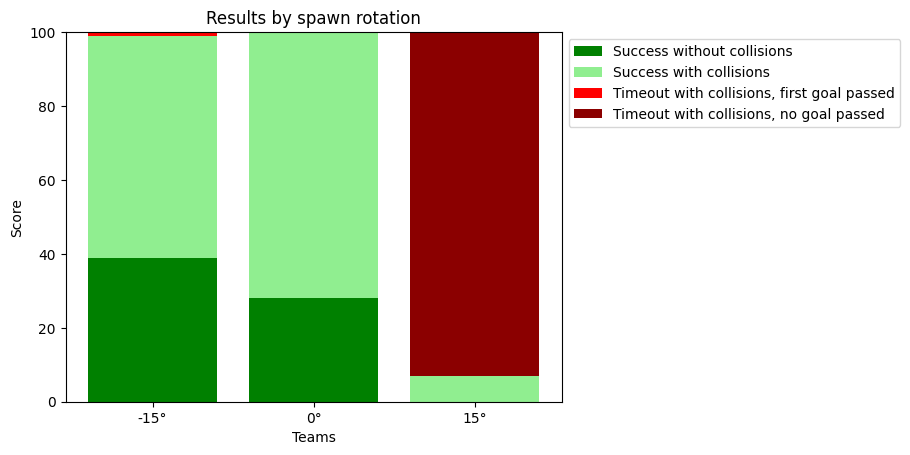
\includegraphics[width=0.8\textwidth]{Bilder/notebook_images/identicalResults_mixedLightSettings.png}
    \caption{Results of 100 episodes for different starting rotations}
    \label{fig:identical_start_conditions_test_result}
\end{figure}


\paragraph{Discussion}

The test shows that identical starting conditions do not always lead to the same episode result. However the success rate is very consistent for the identical starting conditions. The collision rate is significantly less consistent.

The results confirm that the $success\_rates$ of the Basic Evaluation Algorithm are reliable. 


\subsection{Fresh Observations Test}

\ac{HX-P} was trained to not use fresh observations with a fixed step duration of 0.3 seconds. The policy input receives the observation from the start of the previous step as input. The policy input essentially lags 0.3 seconds behind the environment state. This saves processing time during training and evaluation. Alternatively a policy can be run with the $use\_fresh\_obs$ parameter. This makes the policy request a fresh observation from the Unity simulation, see \ref{sec:non_blocking_step_calls}.

The Fresh Observations Test analyses whether switching the trained policy to use fresh observations improves the performance. The policy is evaluated with fresh observations and without fresh observations for each difficulty level using the Basic Evaluation Algorithm \ref{sec:basic_evaluation_algorithm}. The success rates are compared to determine if fresh observations improve the agent's performance.

\paragraph{Results}

\begin{figure}
    \centering
    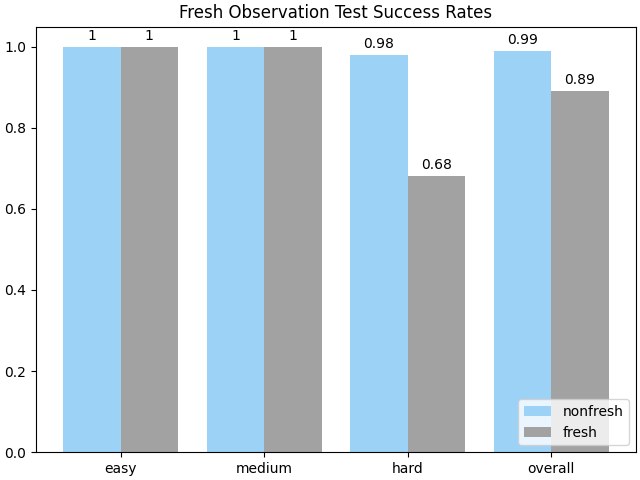
\includegraphics[width=0.8\textwidth]{Bilder/notebook_images/hardDistanceMixedLight_eval_freshNonFresh_success_rates_barplot.png}
    \caption{Success rates for \ac{HX-P} using fresh and non-fresh observations}
    \label{fig:fresh_observations_test_result}
\end{figure}

The results show that the policy performs similar for the easy and medium settings. The success rates are 100\% for both fresh and non-fresh observations. The hard setting shows a strong decrease in performance when using fresh observations. The success rate drops from 98\% to 68\% \ref{fig:fresh_observations_test_result}.

The evaluations using fresh observations also take longer. The Basic Evaluation Algorithm's per call time for the fresh observations is about 20 minutes compared to 17 minutes for the non-fresh observations. The evaluation using fresh observations is slower because the policy has to request a fresh observation from the Unity simulation. This takes additional time.


\paragraph{Discussion}

The policy was trained using non-fresh observations. The policy's performance decreases for hard tracks when it is evaluated using fresh observations.
This suggests that the policy has learned to work with the lag of 0.3 seconds between the environment state and input to the policy. The policy's performance decreases when the lag is removed.

The test confirms that the $use\_fresh\_obs$ parameter should not be changed after the training has been completed.


\subsection{Jetbot Generalization Test}

\ac{HX-P} was trained using the DifferentialJetBot shown in figure \ref{fig:jetbots}. The Jetbot Generalization test evaluates the same policy using the FourWheelJetBot. The policy is only evaluated on the standard light setting to save time.

\paragraph{Results}

\begin{figure}
    \centering
    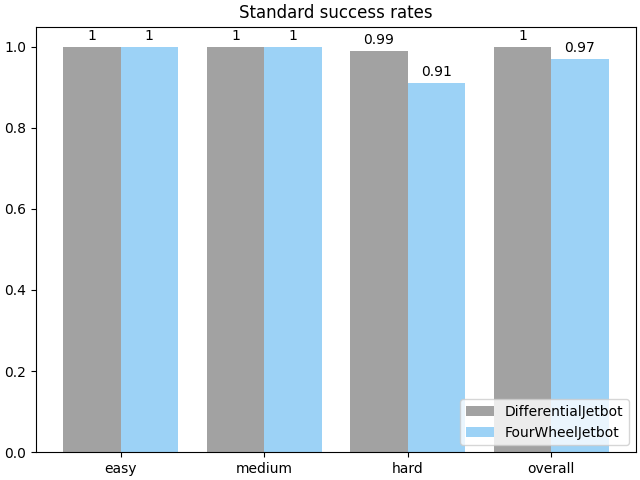
\includegraphics[width=0.45\textwidth]{Bilder/notebook_images/hardDistanceMixedLight_eval_jetbot_generalization_success_rates_barplot.png}
    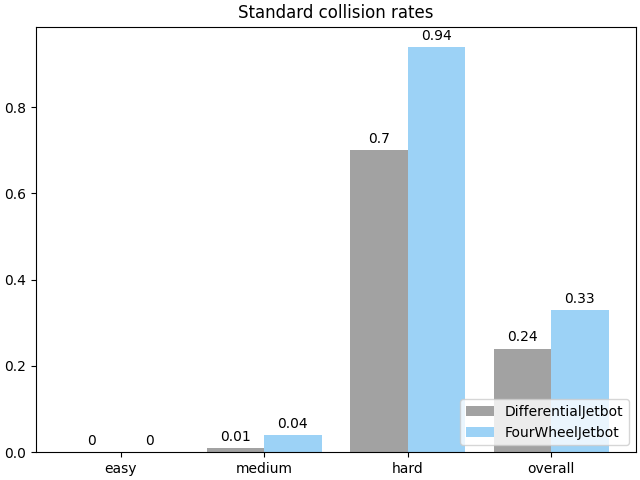
\includegraphics[width=0.45\textwidth]{Bilder/notebook_images/hardDistanceMixedLight_eval_jetbot_generalization_collision_rates_barplot.png}
    \caption{Evaluation of the DifferentialJetBot policy \ac{HX-P} with both jetbot versions}
    \label{fig:result_jetbot_generalization}
\end{figure} % a chart showing the replay outputs

The policy evaluation achieves very high success rates for the FourWheelJetBot with 100\%, 100\% and 91\% for the easy, medium and hard tracks \ref{fig:result_jetbot_generalization}. The collision rates increase for higher difficulties with 0\%, 4\% and 94\%. 
The success and collision rates are slightly worse than on the DifferentialJetBot. The overall success rate of the FourWheelJetBot is 97\% compared to 100\% for the DifferentialJetBot. 

The overall collision rate is 33\% compared to 24\% for the DifferentialJetBot. Especially for the hard tracks the collision rate is much higher for the FourWheelJetBot with 94\% compared to 70\% for the DifferentialJetBot.
The collisions of the DifferentialJetBot were previously described as mainly being minor collisions where the agent scrapes the goal posts with its side. Analysis of the recorded videos shows that the collisions of the FourWheelJetBot are similar. However the agent scrapes the goals on its side for longer durations \ref{sec:fourwheel_collisions}.

% strong collisions here: hard_standard_FourWheelJetBot_env_0_video_2_topview

\paragraph{Discussion}

The policy that was trained on the DifferentialJetBot can be transfered to the FourWheelJetBot with only a slight decrease in performance.
The policy does not have to be retrained in this case. 



\chapter{Conclusion}
\label{cha:Conclusion}

bla conclusion



% Literaturverzeichnis -----------------------------------------------------
%		Das Literaturverzeichnis wird aus der Datenbank erstellt.
%		Die genaue Verwendung von biblatex wird hier jedoch nicht erklärt.
%		Links: 	https://ctan.org/pkg/biblatex?lang=de
%						https://de.overleaf.com/learn/latex/Articles/Getting_started_with_BibLaTeX
% --------------------------------------------------------------------------


\printbibliography

% \setcounter{page}{122}
% \pagenumbering{gobble}
%\pagenumbering{gobble}
\addchap{Erklärung}
Ich versichere, dass ich die vorliegende Arbeit mit dem Thema:

\begin{center}
\textit{\glqq\titel\grqq}\\[1em]
\end{center}
			
selbständig und nur unter Verwendung der angegebenen Quellen und Hilfsmittel angefertigt habe, insbesondere sind wörtliche oder sinngemäße Zitate als solche gekennzeichnet. Mir ist bekannt, dass Zuwiderhandlung auch nachträglich zur Aberkennung des Abschlusses führen kann. Ich versichere, dass das elektronische Exemplar mit den gedruckten Exemplaren übereinstimmt.
\par
\ort, den \eingereicht


\rule[-0.2cm]{5cm}{0.5pt}

\textsc{\autor} 
	% Selbständigkeitserklärung 

% Anhang -------------------------------------------------------------------
%		Die Inhalte des Anhangs werden analog zu den Kapiteln inkludiert.
%		Dies geschieht in der Datei Anhang.tex
% --------------------------------------------------------------------------
\appendix
\clearpage
\renewcommand*{\thesection}{\Alph{section}} 
\pagenumbering{Roman}
%\include{Inhalt/Anhang}



% Index --------------------------------------------------------------------
%		Zum Erstellen eines Index, die folgende Zeile auskommentieren.
% --------------------------------------------------------------------------
%\printindex		% Index hier einfügen
%\ofoot{}
%\include{Inhalt/Thesen}	% Thesen 

\end{document}
